\documentclass[a4paper,twoside,12pt]{book}


\usepackage[T1]{fontenc}
\usepackage[utf8]{inputenc}
\usepackage[italian]{babel}

\usepackage{subfigure}
\usepackage[T1]{fontenc}

\usepackage{fancyhdr}
\usepackage{amsmath}
\usepackage{amssymb}
\usepackage{a4}

\usepackage[pdftex]{graphicx}   
\usepackage{float}  
\graphicspath{{images/}}     
\DeclareGraphicsExtensions{.pdf,.jpeg,.png,.jpg}  
\newcommand{\clearemptydoublepage}{\newpage{\pagestyle{empty}\cleardoublepage}}
\newcommand{\nohyphens}{\hyphenpenalty=10000\exhyphenpenalty=10000\relax}

%% Layout della pagina
%\pagestyle{fancyplain}
%\setlength{\headheight}{14.5pt}
%\addtolength{\headwidth}{\marginparsep}
%\addtolength{\headwidth}{\marginparwidth}
%\renewcommand{\chaptermark}[1]{\markboth{#1}{}}
%\renewcommand{\sectionmark}[1]{\markright{\thesection\  #1}}
%\lhead[\fancyplain{}{\bfseries\thepage}]%
%      {\fancyplain{}{\bfseries\rightmark}}
%\rhead[\fancyplain{}{\bfseries\leftmark}]%
%      {\fancyplain{}{\bfseries\thepage}}
%\cfoot{}

% Questa lunghezza rappresenta la lunghezza completa della pagine, compreso
% lo spazio per le note a margine
%\newlength{\fullpagelen}
%\setlength{\fullpagelen}{\textwidth}
%\addtolength{\fullpagelen}{\marginparsep}
%\addtolength{\fullpagelen}{\marginparwidth}

\makeatletter
\renewenvironment{thebibliography}[1]
  {%
    \chapter*{\bibname}%
    \addcontentsline{toc}{chapter}{\bibname}%
    \@mkboth{\MakeUppercase\bibname}{\MakeUppercase\bibname}%
    \list{\@biblabel{\@arabic\c@enumiv}}%
    {%
      \settowidth\labelwidth{\@biblabel{#1}}%
      \leftmargin\labelwidth
      \advance\leftmargin\labelsep
      \@openbib@code
      \usecounter{enumiv}%
      \let\p@enumiv\@empty
      \renewcommand\theenumiv{\@arabic\c@enumiv}%
    }%
    \sloppy
    \clubpenalty4000
    \@clubpenalty \clubpenalty
    \widowpenalty4000%
    \sfcode`\.\@m%
  }%
  {%
    \def\@noitemerr
    {\@latex@warning{Empty `thebibliography' environment}}%
    \endlist%
  }   % Finisce qui la ridefinizione di thebibliography

\makeatother


\usepackage{color}
\usepackage{listings}

\definecolor{codegreen}{rgb}{0,0.6,0}
\definecolor{codegray}{rgb}{0.5,0.5,0.5}
\definecolor{codepurple}{rgb}{0.58,0,0.82}
\definecolor{backcolour}{rgb}{0.95,0.95,0.92}

\lstdefinestyle{mystyle}{
	backgroundcolor=\color{backcolour},   
	commentstyle=\color{codegreen},
	keywordstyle=\color{magenta},
	numberstyle=\tiny\color{codegray},
	stringstyle=\color{codepurple},
	basicstyle=\footnotesize,
	breakatwhitespace=false,         
	breaklines=true,                 
	captionpos=b,                    
	keepspaces=true,                 
	numbers=left,                    
	numbersep=5pt,                  
	showspaces=false,                
	showstringspaces=false,
	showtabs=false,                  
	tabsize=2
}

\lstset{style=mystyle}




\begin{document}



\pagestyle{fancy}
\renewcommand{\chaptermark}[1]{\markboth{#1}{}}
\renewcommand{\sectionmark}[1]{\markright{\thesection\ #1}}
\fancyhf{} \fancyhead[LE,RO]{\bfseries\thepage}
\fancyhead[LO]{\bfseries\rightmark}
\fancyhead[RE]{\bfseries\leftmark}
\renewcommand{\headrulewidth}{0.5pt}
\renewcommand{\footrulewidth}{0pt}
\fancypagestyle{plain}{
\fancyhead{}
\renewcommand{\headrulewidth}{0pt}}

\thispagestyle{empty}

\begin{center}
  \large
  \textit{UNIVERSIT\'A POLITECNICA DELLE MARCHE\\}
  %\normalsize
  \vspace*{.5cm}
  \textit{ FACOLT\'A DI INGEGNERIA \\}    
\end{center}
%\vspace*{-1.5cm} 
\begin{figure}[h]
	\centering
	
\includegraphics[width=5cm]{logo.png}
\end{figure}
\begin{center}
  \vspace*{0.5cm} 
  \emph{Corso di Laurea Triennale in\\Ingegneria Informatica e dell'Automazione\\}
	\hfill \\
  \vspace*{.75cm} \large %true
  \emph{\textbf{Progettazione e Sviluppo di una Web App per la Gestione di un Orto Botanico}}
  \hfill \\
  \vspace*{.25cm} \large %true
  \emph{\textbf{Design and Development of a Web app to manage a Botanic Garden}}
\end{center}
\vspace*{2.0cm} %\large
\begin{flushleft}
Relatore:\\\textsc{Ch.mo Prof. Mancini Adriano}\\
\end{flushleft}
\vspace*{-2.0cm}
\begin{flushright}
Laureando:\\\textsc{Rossi Andrea}\\      
\end{flushright}
\vspace*{2cm}
\begin{center}
\large{\textsc{Anno Accademico 2019-2020}}
\end{center} \clearpage


\tableofcontents 
\addcontentsline{toc}{chapter}{Elenco delle figure}%

\setcounter{secnumdepth}{3}
\clearemptydoublepage
\chapter{Introduzione}

\section{Obiettivo}
Lo svolgimento di questo progetto è focalizzato sullo sviluppo di una Applicazione Web che consenta di visualizzare piante che sono di interesse nell'ambito di orti botanico in rete.
Quest'ultima deve essere in grado di poter elaborare e visionare dati riguardo quest'ambito, utilizzando specifici linguaggi e software studiati durante il percorso di studio. \newline

\section{Struttura della Tesi}
La tesi viene strutturata principalmente come introduzione all'applicazione web.
Verranno prima affrontati concetti elementari per poi introdurre più nozioni su tali elementi, ogni parte è propedeutica alla successiva.
Viene quindi strutturata come segue:
\begin{itemize}
\item nella prima parte verranno introdotti gli strumenti software e i linguaggi utilizzati suddivisi lato front e back end;
\item nella seconda parte verrà spiegato quali sono state le fasi della progettazione dell'applicazione web. Si parte dal database logic, poi si analizzano gli script php utilizzati nel back end infine il restante codice del front end;
\item nella terza parte  vengono espletati tutti gli accorgimenti necessari affinché si abbia un corretto set-up dell'applicazione web; 
\item nella quarta parte verranno espletati altri accorgimenti affinché si abbia la migliore esperienza di navigazione mobile dal browser Safari. Dopodiché verrà fatta una panoramica dell'applicazione web, guidando l'utente tramite l'uso di screen;
\item nell'ultima parte verranno esposte le conclusioni e verranno introdotti gli sviluppi futuri;
\end{itemize}
\section{La scelta dell'Applicazione Web}
La scelta dell'applicazione web anziché un'applicazione software scritta in Java o C\# è motivata dal fatto che essenzialmente un'applicazione web può essere eseguita su qualunque dispositivo dotato di un web browser. Altrimenti il percorso di sviluppo doveva essere suddiviso a seconda del dispositivo, quindi utilizzando Android Studio per un dispositivo Android, Xcode per un dispositivo Apple e via dicendo. \newline
\section{Indipendenza da software esterni per la gestione del database}
Una cosa di fondamentale importanza che è stata implementata con successo in questo progetto è l'indipendenza da un modulo esterno per la gestione del database ad eccezione della creazione del database, tabelle e dati di default.
Tale scelta comporta una maggiore flessibilità ed anche facilità per la visualizzazione e manipolazione dei dati del database senza dover ogni volta accedere a un client di gestione di basi di dati o al modulo PhpMyAdmin.

\section{La scelta di impiegare due Front-end}
Sono stati realizzati due front-end che consumano lo stesso back-end. \newline
Il front-end \textbf{basic} come suggerisce il nome, è più basilare, è privo di effetti grafici e rispecchia una interfaccia web light. \newline
Il front-end \textbf{full} invece è completo anche dal punto di vista grafico. Rispecchia gli standard attuali \textit{Material Design} dell'odierna programmazione web.
\newline \newline
Concludendo si può dire che sviluppare due front end è stato un ottimo esercizio per raggiungere gli stessi obiettivi utilizzando linguaggi di programmazione, costrutti ed approcci diversi per ogni front end. 


 \clearemptydoublepage
\chapter{Strumenti utilizzati}

\section{Front-end e back-end}
I termini front end (in sigla \textbf{ FE}) e back end (in sigla \textbf{BE}) denotano, rispettivamente, la parte visibile all'utente e con cui egli può interagire (interfaccia utente) e la parte che permette l'effettivo funzionamento di queste interazioni.
Il front end, è responsabile dell'acquisizione dei dati di ingresso e della loro elaborazione tali da renderli utilizzabili dal back end. \newline
Nella programmazione e sviluppo dei siti web viene definito front end la parte visibile da chiunque e raggiungibile all'indirizzo web del sito e viene definita back end la parte di amministrazione di un sito accessibile solo da amministratori del sito web. Front end e back end si utilizzano solamente quando il sito web è dinamico \cite{sito_frontback_end}. 


\section{Back End}

\subsection{Software}
Di seguito saranno introdotti vari strumenti software che hanno trovato ampio utilizzo per la realizzazione di questo progetto.
\subsubsection{Web Server}
Un server web (o web server) è un'applicazione software che, in esecuzione su un server, è in grado di gestire le richieste di trasferimento di pagine web di un client, tipicamente un web browser. La comunicazione tra server e client avviene tramite il protocollo \textbf{HTTP}, che utilizza la porta TCP 80 (o 8080), o eventualmente la versione sicura \textbf{HTTPS}, che utilizza invece la 443 \cite{sito_webserver}.
\newline
\newline
\newline
In questo progetto è stato utilizzato \textbf{Apache HTTP Server}.
Il Web Server Apache presenta un'architettura modulare, quindi ad ogni richiesta del client vengono svolte funzioni specifiche da ogni modulo di cui è composto, come unità indipendenti. Ciascun modulo si occupa di una funzionalità, ed il controllo è gestito dal core.
In linea continua il flusso dei dati reale
Tratteggiato il flusso dei dati astratto che forma la pipeline
Al di sopra del ciclo del core un demone esegue un ciclo di polling, attraverso il quale vengono interrogate continuamente le linee logiche da cui possono pervenire messaggi di richiesta.
Il core passa poi la richiesta ai vari moduli in modo sequenziale, usando i parametri di uscita di un modulo come parametri di accesso per il successivo, creando così l'illusione di una comunicazione orizzontale fra i moduli (Pipeline software) \cite{sito_apache}.
Le principali fasi di cui è composto il ciclo sono:
\begin{itemize}
\item \textbf{Translation}: traduce la richiesta del client
\textbf{Access Control}: controlla le richieste in base ai criteri di autorizzazione.
\item \textbf{MIME Type}: identifica il tipo di contenuto e decide quali moduli possono contribuire a servire la richiesta.
\item \textbf{Response}: invia la risposta al client e attiva eventuali procedure.
\item \textbf{Logging}: tiene traccia di tutto ciò che è stato fatto.
\end{itemize}

 \begin{figure}[h]
	\centering
	\caption {Architettura di Apache : In linea continua il flusso dei dati reale,
		tratteggiato il flusso dei dati astratto che forma la pipeline \cite{sito_apache}.}
	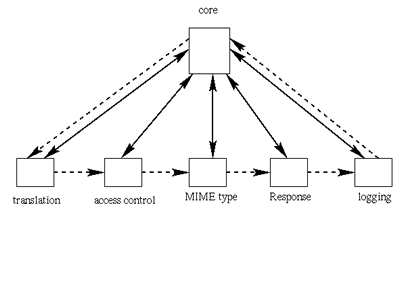
\includegraphics[scale = 0.8]{apache.png}
\end{figure}

\newpage

\subsubsection{Database Management System}
Un Database Management System, abbreviato in \textbf{DBMS} o Sistema di gestione di basi di dati, è un sistema software progettato per consentire la creazione, la manipolazione e l'interrogazione efficiente di database e ospitato su architettura hardware dedicata oppure su semplice computer \cite{sito_dbms}.\newline \newline
In questo progetto viene utilizzato \textbf{MySQL} che è un Relational database management system (\textbf{RDBMS}) composto da un client a riga di comando e un server. Entrambi i software sono disponibili sia per sistemi Unix e Unix-like sia per Windows.
\newline
MySQL è un software libero rilasciato a doppia licenza, compresa la GNU General Public License, ed è sviluppato per essere il più possibile conforme agli standard ANSI SQL e ODBC SQL \cite{sito_mysql_license}.
\newline
I sistemi e i linguaggi di programmazione che supportano MySQL sono molto numerosi: ODBC, Java, Mono, .NET, PHP, Python e molti altri.
\newline
In MySQL una tabella può essere di diversi tipi (o \textbf{storage engine}). Ogni tipo di tabella presenta proprietà e caratteristiche differenti (transazionale o meno, migliori prestazioni, diverse strategie di locking, funzioni particolari, ecc). 
Degna di nota è sicuramente il tipo di tabella \textbf{InnoDB} \cite{sito_innodb},
che mette a  disposizione le seguenti funzionalità:
\begin{itemize}
\item transazioni SQL con savepoint e transazioni XA;
\item lock a livello di record;
\item chiavi esterne (\textbf{Foreign Key});
\item buffer per gli indici, le chiavi, modifiche, cancellazioni;
\item compressione delle tabelle;
\item Il lock in InnoDB per quanto riguarda i comandi SELECT è di tipo non-locking. InnoDB offre delle ottime performance in termini di prestazioni e utilizzo della CPU.
\end{itemize}
Per quanto riguarda i limiti di questo tipo di tabella, si ha:
\begin{itemize}
\item Impossibilità creare più di 1000 colonne per tabella;
\item Su alcuni sistemi operativi le dimensioni del tablespace non possono superare i 2 GB;
\item La grandezza di tutti i file di log di InnoDB deve essere inferiore ai 4 GB;
\item	La grandezza minima di un tablespace è di 10 MB;
\item	Gli indici FULLTEXT sono stati introdotti nella versione 5.6 di MySQL e nella versione 10.0 di MariaDB, ma in alcune circostanze sono meno efficienti rispetto a quelli di \textbf{MyISAM} (storage engine predefinito in MySQL dalla sua introduzione (versione 3.23) fino alla versione 5.5).
\end{itemize}

\subsubsection{PhpMyAdmin}

PhpMyAdmin è un'applicazione web scritta in PHP, distribuita con licenza GPL, che consente di amministrare un database MySQL o MariaDB tramite un qualsiasi browser. 
\newline
PhpMyAdmin permette di creare un database da zero, creare le tabelle ed eseguire operazioni di ottimizzazione sulle stesse. Sono previste delle funzionalità per l'inserimento dei dati (popolazione del database), per le query, per il backup dei dati, e molto altro  \cite{sito_phpmyadmin}.
\newline


\subsubsection{XAMPP}
XAMPP è una piattaforma software multi-piattaforma e libera costituita da Apache HTTP Server, il gestore di database MariaDB (prima della versione 5.5.30 il gestore di database era MySQL)  e tutti gli strumenti necessari per utilizzare i linguaggi di programmazione PHP e Perl. Il nome è un acronimo dei software sopra citati (la X sta per x-platform, l'abbreviazione di cross-platform in lingua inglese ovvero multipiattaforma) \cite{sito_xampp}.
I componenti inclusi in questo pacchetto e utilizzati sono:
\begin{itemize}
\item il web server: \textbf{Apache} HTTP Server;
\item il database management system : \textbf{MariaDB} e SQLite; 
\item come linguaggio di programmazione: \textbf{PHP};
\item come modulo \textbf{PhpMyadmin}.
\end{itemize}


 \begin{figure}[h]
	\centering
	\caption{Pannello di XAMPP per Windows}
	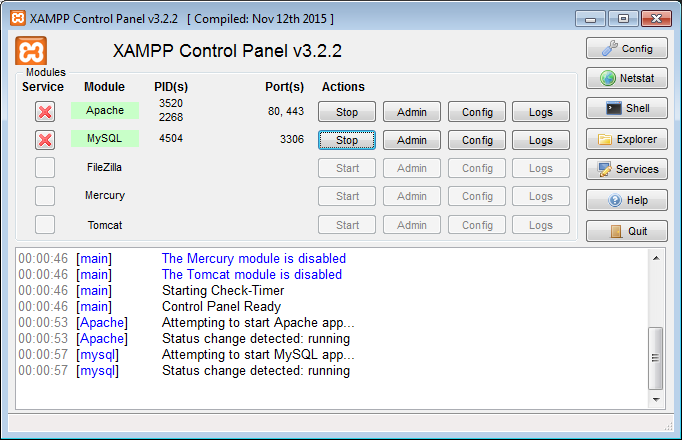
\includegraphics[scale = 0.8]{xampp.png}
\end{figure}

\newpage

\subsection{Linguaggi di Programmazione}
Verranno ora introdotti i linguaggi di programmazione utilizzati nella parte di \textbf{BE}.
\subsubsection{PHP}
Il PHP (acronimo ricorsivo di "PHP: Hypertext Preprocessor", preprocessore di ipertesti; originariamente acronimo di "Personal Home Page") è un linguaggio di scripting interpretato, originariamente concepito per la programmazione di pagine web dinamiche. L'interprete PHP è un software libero distribuito sotto la PHP License.
\newline
PHP è in grado di interfacciarsi a innumerevoli DBMS tra cui MySQL \cite{sito_php}. 

\subsubsection{SQL}
L' SQL (Structured Query Language) è un linguaggio standardizzato per database basati sul modello relazionale (RDBMS) progettato per: 
\begin{itemize}
\item creare e modificare schemi di database (DDL - Data Definition Language);
\item inserire, modificare e gestire dati memorizzati (DML - Data Manipulation Language);
\item interrogare i dati memorizzati (DQL - Data Query Language);
\item creare e gestire strumenti di controllo ed accesso ai dati (DCL - Data Control Language). 
\end{itemize}
SQL è un linguaggio per interrogare e gestire basi di dati mediante l'utilizzo di costrutti di programmazione denominati query. Con SQL si leggono, modificano, cancellano dati e si esercitano funzioni gestionali ed amministrative sul sistema dei database \cite{sito_sql}. 
Esso si divide in:
\begin{itemize}
\item Data Definition Language (DDL) - permette di creare e cancellare database o di modificarne la struttura;
\item Data Manipulation Language (DML) - permette di inserire, cancellare, modificare i dati;
\item Data Control Language (DCL) - permette di gestire gli utenti e i permessi;
\item Query language (QL) - permette di interrogare il database, cioè di leggere i dati;
\item Device Media Control Language (DMCL) - permette di controllare i supporti (memorie di massa) dove vengono memorizzati i dati.
\end{itemize}
\newpage

\section{Front End}
\subsection{Software}
\subsubsection{Web Browser}
Il web browser (o più semplicemente browser) è un'applicazione per il recupero, la presentazione e la navigazione di risorse sul web. Tali risorse (come pagine web, immagini o video) sono messe a disposizione sul World Wide Web (la rete globale che si appoggia su Internet), su una rete locale o sullo stesso computer dove il browser è in esecuzione. 
Nell'architettura di rete \textbf{client-server} di Internet il browser rappresenta dunque il client che fa richieste di risorse web ai vari web server e application server ospitanti rispettivamente siti web e applicazioni web. Esso rappresenta dunque il sistema software di interfacciamento dell'utente con la rete che rende la navigazione dell'utente tipicamente user-friendly, sebbene ai primordi della rete siano esistiti anche browser testuali da riga di comando su shell. I browser vengono principalmente utilizzati su personal computer, ma anche su altri dispositivi che consentono la navigazione in Internet, come i palmari e gli smartphone. Quelli più noti e diffusi sono Internet Explorer, Mozilla Firefox, Google Chrome, Safari, Opera e Internet Explorer \cite{sito_web_browser}.
\newline \newline
In questo progetto viene utilizzato \textbf{Mozilla Firefox} che è un web browser libero e multipiattaforma, mantenuto da Mozilla Foundation per la navigazione da desktop e il web browser \textbf{Safari} sviluppato dalla Apple Inc per i sistemi operativi iOS e macOS per la navigazione da mobile.

\subsubsection{Editor}
Viene utilizzato \textbf{Visual Studio Code} che è un editor di codice sorgente sviluppato da Microsoft per Windows, Linux e macOS. Esso include supporto per debugging, un controllo per Git integrato, Syntax highlighting, IntelliSense, Snippet e refactoring del codice. È anche personalizzabile: gli utenti possono cambiare il tema dell'editor, le scorciatoie da tastiera, e le preferenze. È un software libero, anche se la versione ufficiale è sotto una licenza proprietaria \cite{sito_visual_studio_code}.
\newline
Questo editor supporta la colorazione della sintassi per i linguaggi utilizzati nel progetto (\textbf{Syntax highlighting}) come è possibile vedere nella seguente immagine.

 \begin{figure}[H]
	\centering
	\caption{script php (config.php) per la connessione al database}
	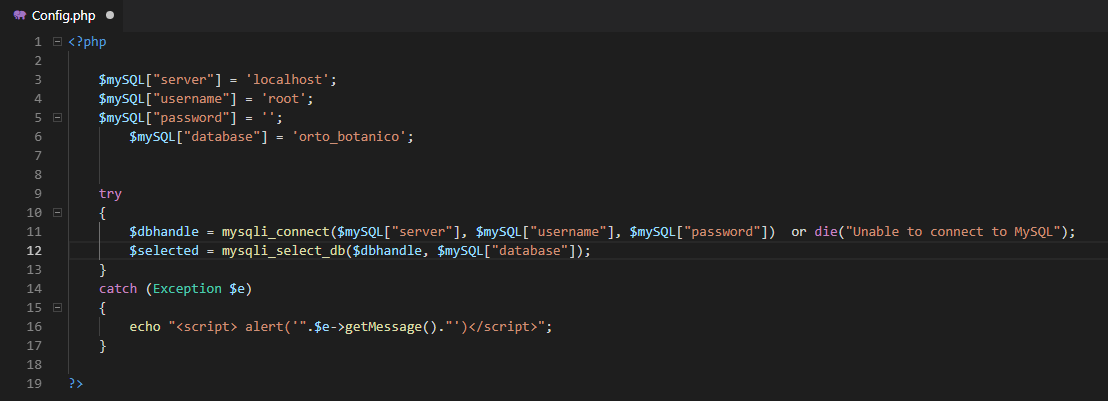
\includegraphics[width= 13cm]{visual_studio_code.png}
\end{figure}

\subsubsection{Leaflet}
Leaflet è una libreria JavaScript per sviluppare mappe geografiche interattive (WebGIS). Sviluppato dal 2010, supporta la maggior parte dei browser e degli standard HTML5 e CSS3. Permette di mostrare punti di interesse, linee o aree, o strutture dati come file GeoJSON, o livelli interattivi, su una mappa a tasselli \cite{sito_leaflet}. \newline
Punti di interesse (markers) e livelli (layers) possono essere aggiunti successivamente, in questo progetto viene fatta ampio uso di questa metodologia, aggiungendo e rimuovendo dinamicamente punti di interesse.
\begin{figure}[h]
	\centering
	\caption{immagine raffigurante dei punti di interesse: è possibile vedere il \textbf{polygon} che raffigura l'orto botanico \textit{Parco UNIVPM} con al centro un \textbf{circle} che cliccato apre il tooltip e i due \textbf{markers} che raffigurano i beacon (piante) nel parco.}
	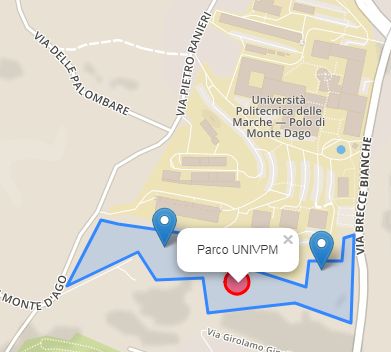
\includegraphics[width= 8cm]{leaflet.png}
\end{figure}

\subsubsection{W3C Geolocation API}
La W3C Geolocation API è una libreria del World Wide Web Consortium (W3C) per standardizzare un'interfaccia per recuperare le informazioni sulla posizione geografica di un dispositivo lato client. Le fonti più comuni di informazione sulla posizione dell'utente vengono stimate tramite :
\begin{itemize}
\item indirizzo IP;
\item Wi-Fi;
\item indirizzo MAC Bluetooth;
\item identificazione radio-frequenza (RFID);
\item posizione della connessione Wi-Fi;
\item Global Positioning System (GPS);
\item ID cella GSM / CDMA.
\end{itemize} 
La posizione dell'utente verrà restituita con una precisione determinata in base alla migliore fonte di informazione sulla posizione disponibile \cite{sito_geolocation_API}.

\subsubsection{WebRTC API}
WebRTC (Web Real-Time Communications) è una tecnologia che consente alle applicazioni Web e ai siti di acquisire e, a scelta, trasmettere contenuti audio e / o video, nonché di scambiare dati arbitrari tra browser senza richiedere un intermediario. L'insieme di standard che comprende WebRTC consente di condividere dati ed eseguire teleconferenze peer-to-peer, senza richiedere che l'utente installi plug-in o qualsiasi altro software di terze parti \cite{sito_WebRTC_API} \cite{sito_WebRTC_esempi}.

\newpage

\subsection{Linguaggi Utilizzati}
\subsubsection{HTML}
L'HyperText Markup Language è un \textbf{linguaggio di markup} che descrive le modalità di impaginazione o visualizzazione grafica (layout) del contenuto, testuale e non, di una pagina web attraverso tag di formattazione. Sebbene l'HTML supporti l'inserimento di script e oggetti esterni quali immagini o filmati, non è un linguaggio di programmazione: non prevedendo alcuna definizione di variabili, strutture dati, funzioni o strutture di controllo che possano realizzare programmi, il suo codice è in grado soltanto di strutturare e decorare dati testuali.
Quando un documento ipertestuale scritto in HTML è memorizzato in un file la sua estensione è tipicamente \textbf{.html} o \textbf{.htm}.
I documenti HTML vengono immagazzinati sui dischi rigidi di macchine elaboratrici (computer-server) costantemente collegate e connesse alla rete Internet. Su queste macchine è installato un software specifico (web server) che si occupa di produrre e inviare i documenti ai browser degli utenti che ne fanno richiesta usando il protocollo HTTP per il trasferimento dati \cite{sito_HTML}.

\subsubsection{CSS}

Il CSS (acronimo di Cascading Style Sheets, in italiano fogli di stile a cascata), è un linguaggio usato per definire la \textbf{formattazione} di documenti HTML, XHTML e XML. Le regole per comporre il CSS sono contenute in un insieme di direttive (Recommendations) emanate a partire dal 1996 dal W3C.
L'introduzione del CSS si è resa necessaria per separare i contenuti delle pagine HTML dalla loro formattazione e permettere una programmazione più chiara e facile da utilizzare, sia per gli autori delle pagine stesse sia per gli utenti, garantendo contemporaneamente anche il riutilizzo di codice ed una sua più facile manutenzione \cite{sito_CSS}.
Nessun browser attuale offre il supporto completo e corretto delle specifiche CSS. Tuttavia esistono browser che si avvicinano molto a questo risultato ed altri che invece ne sono molto lontani. La lista che segue è di motori di rendering perché a loro è assegnato il compito di formattare la pagina secondo le istruzioni CSS.

\subsubsection{CSS Framework CSS}
Un framework CSS è un software predisposto per consentire un web design più semplice e conforme agli standard utilizzando il linguaggio CSS. La maggior parte di questi framework contiene almeno una griglia. I framework più funzionali includono anche più funzionalità e funzioni aggiuntive basate su JavaScript e JQuery, ma sono principalmente orientati al design e non invadenti. \newline
Due esempi ampiamente utilizzati sono Bootstrap e \textbf{Materialize} (utilizzato in questo progetto) \cite{sito_framework_css}.

\subsubsection{Javascript}
JavaScript è un linguaggio di scripting orientato agli oggetti e agli eventi, comunemente utilizzato nella programmazione Web lato client per la creazione, in siti web e applicazioni web, di effetti dinamici interattivi tramite funzioni di script invocate da eventi innescati a loro volta in vari modi dall'utente sulla pagina web in uso (mouse, tastiera, caricamento della pagina ecc...).
\newline
Tali funzioni di script, utilizzati dunque nella logica di presentazione, possono essere opportunamente inserite in file HTML, in pagine JSP o in appositi file separati con estensione .js poi richiamati nella logica di business. 
\newline
Un uso principale del JavaScript in ambito Web è la scrittura di piccole funzioni integrate nelle pagine HTML che interagiscono con il DOM del browser per compiere determinate azioni non possibili con il solo HTML statico: controllare i valori nei campi di input, nascondere o visualizzare determinati elementi, ecc.
\newline
Sfortunatamente, gli standard DOM imposti dal W3C non sempre vengono rispettati dai vari browser: browser diversi (anche a seconda del loro motore di rendering) espongono diversi oggetti o metodi allo script (Internet Explorer è solito aderire agli standard con piccole modifiche, e tratta ad esempio l'oggetto event come globale), ed è quindi spesso necessario implementare controlli aggiuntivi ad una funzione JavaScript, per garantirne la compatibilità con ciascun browser \cite{sito_Js}.

\subsubsection{JQuery}
JQuery è una libreria JavaScript per applicazioni web. Nasce con l'obiettivo di semplificare la selezione, la manipolazione, la gestione degli eventi e l'animazione di elementi DOM in pagine HTML, nonché implementare funzionalità \textbf{AJAX} \cite{sito_JQuery}.

\subsubsection{AJAX}
AJAX, acronimo di Asynchronous JavaScript and XML, è una tecnica di sviluppo software per la realizzazione di applicazioni web interattive (Rich Internet Application). Lo sviluppo di applicazioni HTML con AJAX si basa su uno scambio di dati in background fra web browser e server, che consente l'aggiornamento dinamico di una pagina web senza esplicito ricaricamento da parte dell'utente.
\newline
La tecnica AJAX utilizza una combinazione di:
\begin{itemize}
	\item HTML (o XHTML) e CSS per il markup e lo stile;
	\item DOM (Document Object Model) manipolato attraverso un linguaggio ECMAScript come JavaScript o JScript per mostrare le informazioni ed interagirvi;
	\item l'oggetto XMLHttpRequest per l'interscambio asincrono dei dati tra il browser dell'utente e il web server. In alcuni framework AJAX e in certe situazioni, può essere usato un oggetto Iframe invece di XMLHttpRequest per scambiare i dati con il server e, in altre implementazioni, tag <script> aggiunti dinamicamente (JSON);
	\item in genere viene usato XML come formato di scambio dei dati, anche se di fatto qualunque formato può essere utilizzato, incluso testo semplice, HTML preformattato, JSON e perfino EBML. Questi file sono solitamente generati dinamicamente da script lato server. 
\end{itemize}
AJAX non è una tecnologia individuale, quanto piuttosto un gruppo di tecnologie utilizzate insieme.
\newline
Le applicazioni web che usano AJAX richiedono browser che supportano le tecnologie necessarie (quelle dell'elenco sopra). \newline Questi browser includono: Firefox, Opera, Konqueror, Safari, Internet Explorer e Chrome. Tuttavia, per specifica, \textit{Opera non supporta la formattazione degli oggetti XSL} \cite{sito_Ajax}.
 \clearemptydoublepage
\chapter{Progettazione e Sviluppo}

In questo capitolo verrà trattato l'approccio utilizzato per sviluppare dalle fondamenta l'applicazione web. Verrà quindi spiegato passo passo come è stata realizzata l'applicazione web e verranno forniti i codici utilizzati per una maggiore chiarezza. \newline
Si parte analizzando il livello di back-end più alto, quello del database.
\section{Database Logic}

\subsubsection{Contesto e Esigenze del Database}
Il database deve rappresentare astrattamente la situazione che si sta studiando. Essendo un orto botanico composto essenzialmente dalle piante, si parte da quest'entità a sviluppare il modello della base di dati.
La logica che c'è a questo livello prevede che una pianta sia di una data specie e che idealmente abbia un dispositivo elettronico per permettere l'interazione telematica (beacon). Queste piante faranno parte di un dato sito botanico ed è infatti qua che nasce una rappresentazione astratta di tipo n:m tra pianta e sito. \newline
Un'esigenza del database riguarda l'engine utilizzato per le tabelle, che è del tipo \textbf{InnoDB}, dato che si fa ampio uso delle chiavi esterne (\textit{foreign keys}).
Tali Foreign Keys permettono al meglio di realizzare una base di dati astratta conforme alla realtà di nostro interesse.
\newline 




\subsection{Modello E-R}
\begin{figure}[H]
	\centering
	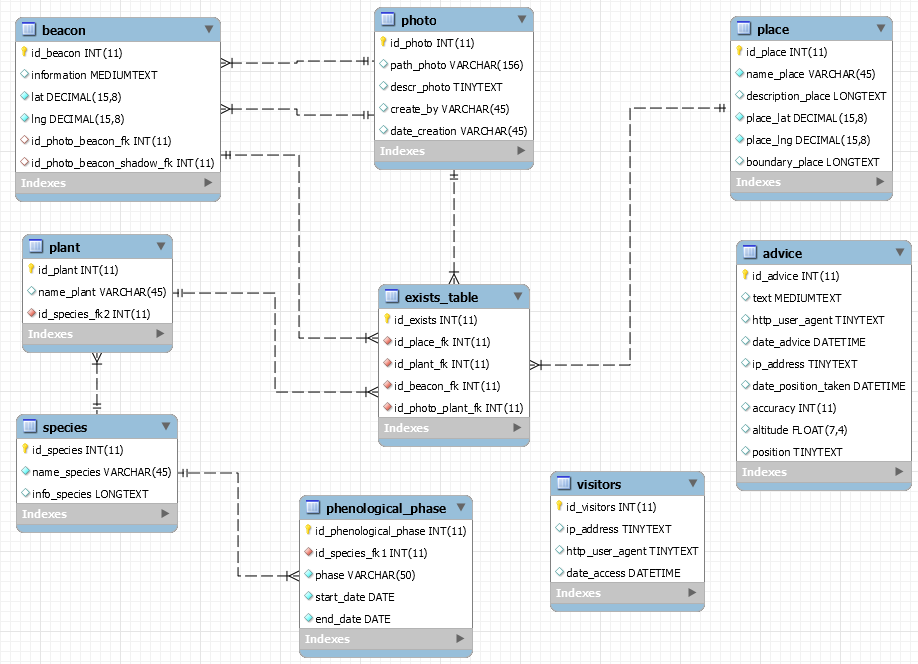
\includegraphics[width= 15cm]{DB.png}
\end{figure}




\subsection{Tabelle}
Di seguito verranno analizzate e spiegate, una ad una tutte le tabelle utilizzate nella base di dati.

\subsubsection{Photo}


Questa tabella rappresenta i contenuti multimediali che vengono caricati dinamicamente nel web server. \newline
È composta da:
\begin{itemize}
\item \textbf{id\_photo} : chiave primaria univoca intera, not null e auto incrementante per distinguere univocamente ogni oggetto registrato nel database;

\item \textbf{path\_photo} : il percorso dell'oggetto multimediale nel nostro server, questa colonna è unique, dato che non possono esserci due oggetti con lo stesso percorso;

\item \textbf{descr\_photo} : la descrizione dell'oggetto caricato;

\item \textbf{create\_by} : campo che indica da chi è stato inserito l'oggetto nel server;

\item \textbf{date\_creation} : la data di inserimento, nel formato YYYY-MM-DD hh:mm:ss.
\end{itemize}
 
 \begin{lstlisting}[language=SQL, caption=Codice SQL della Tabella Photos]
 CREATE TABLE `photo` (
 `id_photo` int(11) NOT NULL AUTO_INCREMENT,
 `path_photo` varchar(156),
 `descr_photo` tinytext, 
 `create_by` varchar(45),
 `date_creation` varchar(45),
 PRIMARY KEY (`id_photo`),
 UNIQUE (`path_photo`)
 ) ENGINE=InnoDB;
 \end{lstlisting}
 
\subsubsection{Beacon}

Questa Tabella rappresenta i beacon nella nostra mappa.
Ci sono due chiavi esterne che fanno referenza alla tabella photo.
\newline Troviamo le seguenti colonne:

\begin{itemize}
\item \textbf{id\_beacon} : chiave primaria univoca intera, not null e auto incrementante per distinguare univocamente ogni beacon registrato nel database;
\item \textbf{information} : informazioni sul beacon;
\item \textbf{lat} : la latitudine, non può essere null;
\item \textbf{lng} : la longitudine, non può essere null;
\item \textbf{id\_photo\_beacon\_fk}: chiave esterna che può anche essere null. In tal caso il beacon avrà l'immagine di default, diversamente si avrà l'immagine specificata;
\item \textbf{id\_photo\_beacon\_shadow\_fk} : chiave esterna che può anche essere null. In tal caso il beacon avrà l'immagine ombra di default, diversamente si avrà l'immagine specificata.
\end{itemize}

\begin{lstlisting}[language=SQL, caption=Codice SQL della Tabella Beacon]

CREATE TABLE `beacon` (
`id_beacon` int(11) NOT NULL AUTO_INCREMENT,
`information` mediumtext,
`lat` decimal(15,8) NOT NULL,
`lng` decimal(15,8) NOT NULL,
`id_photo_beacon_fk` int(11) DEFAULT NULL,
`id_photo_beacon_shadow_fk` int(11) DEFAULT NULL,
PRIMARY KEY (`id_beacon`),
CONSTRAINT `id_photo_beacon_fk` FOREIGN KEY (`id_photo_beacon_fk`) REFERENCES `photo` (`id_photo`) ON UPDATE CASCADE,
CONSTRAINT `id_photo_beacon_shadow_fk` FOREIGN KEY (`id_photo_beacon_shadow_fk`) REFERENCES `photo` (`id_photo`) ON UPDATE CASCADE
) ENGINE=InnoDB;

\end{lstlisting}

\subsubsection{Species}
Questa Tabella indica le specie degli alberi dei nostri orti di interesse. \newline È formata dalle colonne:
\begin{itemize}
\item \textbf{id\_species} : chiave primaria univoca intera, not null e auto incrementante per distinguere univocamente ogni specie registrata nel database;

\item \textbf{name\_species} : il nome della specie;

\item \textbf{info\_species} : informazioni degne di nota sulla specie;
\end{itemize}

\begin{lstlisting}[language=SQL, caption=Codice SQL della Tabella Species]
CREATE TABLE `species` (
`id_species` int(11) NOT NULL AUTO_INCREMENT,
`name_species` varchar(45) NOT NULL,
`info_species` longtext,
PRIMARY KEY (`id_species`)
) ENGINE=InnoDB;
\end{lstlisting}

\subsubsection{Phenological Phase}
Questa tabella rappresenta le possibili fasi fenologiche delle specie registrata nel database. Ha una chiave esterna che la collega con la tabella \textbf{species}. \newline
È formata dalle colonne:
\begin{itemize}
\item \textbf{id\_phenological\_phase} : chiave primaria univoca intera, not null e auto incrementante per distinguare univocamente ogni fase fenologica registrato nel database;
\item  \textbf{id\_species\_fk1} : chiave esterna che fa riferimento a id\_species e server per capire quale specie ha una data fase fenologica;
\item  \textbf{phase} : la fase fenologica;
\item  \textbf{start\_date} l'inizio della fase fenologica in formato YYYY-MM-DD;
\item  \textbf{end\_date}.
\end{itemize} 
Tutte le colonne sono not null. È importante far notare che se si vuole registrare una fase fenologica che scavalchi l'anno, non è possibile farlo con un solo record (es: inizio 1 Dicembre, fine 1 Febbraio) ma si inseriscono due record spezzandoli alla fine dell'anno come segue : 
\begin{itemize}
\item inizio 1 Dicembre, fine 31 Dicembre;
\item inizio 1 Gennaio , fine 1 Febbraio.
\end{itemize}

\begin{lstlisting}[language=SQL, caption=Codice SQL della Tabella Phenological Phase]
CREATE TABLE `phenological_phase` (
`id_phenological_phase` int(11) NOT NULL AUTO_INCREMENT,
`id_species_fk1` int(11) NOT NULL,
`phase` varchar(50) NOT NULL,
`start_date` date NOT NULL,
`end_date` date NOT NULL,
PRIMARY KEY (`id_phenological_phase`),
CONSTRAINT `id_species_fk1` FOREIGN KEY (`id_species_fk1`) REFERENCES `species` (`id_species`) ON UPDATE CASCADE
) ENGINE=InnoDB;
\end{lstlisting}

\subsubsection{Place}
Questa tabella rappresenta gli orti botanici. \newline
È formata dalle colonne:
\begin{itemize}
\item \textbf{id\_place} : chiave primaria univoca intera, not null e auto incrementante per distinguare univocamente ogni place registrato nel database;
\item \textbf{name\_place} : nome del place. Non possono esserci duplicati del nome dato che ha attrbuto unique;
\item \textbf{description\_place} : descrizione del place;		
\item \textbf{place\_lat} : latitudine del place;
\item \textbf{place\_lng} : longitudine del place;
\item \textbf{boundary\_place}: insieme cordinate che permettono a leaflet di disegnare l'elemento sulla mappa, questa colonna è di tipo longtext.
\end{itemize}

\begin{lstlisting}[language=SQL, caption=Codice SQL della Place Photos]

CREATE TABLE `place` (
`id_place` int(11) NOT NULL AUTO_INCREMENT,
`name_place` varchar(45) NOT NULL,
`description_place` longtext,
`place_lat` decimal(15,8) NOT NULL,
`place_lng` decimal(15,8) NOT NULL,
`boundary_place` longtext,
PRIMARY KEY (`id_place`),
UNIQUE (`name_place`)
) ENGINE=InnoDB;

\end{lstlisting}

\subsubsection{Plant}
Questa tabella rappresenta una pianta. È collegata tramite chiave esterna alla tabella species. \newline
È formata dalle colonne:
\begin{itemize}
\item \textbf{id\_plant} : chiave primaria univoca intera, not null e auto incrementante per distinguare univocamente ogni pianta registrata nel database;
\item \textbf{name\_plant} : nome fittizio della pianta;
\item \textbf{id\_species\_fk2} : chiave esterna che indica la specie della pianta.
\end{itemize}
Da notare che la colonna \textit{id\_species} della tabella \textit{species} viene referenziata due volte, per evitare di incorrere nell'errore \textbf{Duplicate key on write or update} si distinguono rispettivamente \textbf{id\_species\_fk1} e \textbf{id\_species\_fk2}.

\begin{lstlisting}[language=SQL, caption=Codice SQL della Tabella Plant]
CREATE TABLE `plant` (
`id_plant` int(11) NOT NULL AUTO_INCREMENT,
`name_plant` varchar(45) DEFAULT NULL,
`id_species_fk2` int(11) NOT NULL,
PRIMARY KEY (`id_plant`),
CONSTRAINT `id_species_fk2` FOREIGN KEY (`id_species_fk2`) REFERENCES `species` (`id_species`) ON UPDATE CASCADE 
) ENGINE=InnoDB; 
\end{lstlisting}

\subsubsection{exists\_table}
Un record di questa tabella indica effettivamente che esiste una pianta, in un dato orto dove è stato posizionato un beacon. \newline
Per fare ciò, questa tabella ha come chiave esterna la chiave primaria della tabella \textbf{beacon} e dato che funge da appoggio alla relazione \underline{n:m} tra le tabelle \textbf{plant} e \textbf{place} conterrà le loro chiavi primarie come chiavi esterne. \newline

È quindi formata dalle seguenti colonne:

\begin{itemize}
\item \textbf{id\_exists} : chiave primaria univoca intera, not null e auto incrementante per distinguare univocamente ogni esistenza di un elemento di interesse completo, localizzabile nella mappa, registrato nel database;
\item \textbf{id\_place\_fk} : chiave esterna che fa riferimento a un dato place;
\item \textbf{id\_plant\_fk} : chiave esterna che fa riferimento a una data pianta;
\item \textbf{id\_beacon\_fk} : chiave esterna che fa riferimento a un dato beacon;
\item \textbf{id\_photo\_plant\_fk} : chiave esterna che fa riferimento alla foto della pianta.

\end{itemize}
Da notare che non è possibile chiamare la tabella solamente \textbf{exists}, dato che in SQL è una parola chiave.
\begin{lstlisting}[language=SQL, caption=Codice SQL della Tabella exists\_table]

CREATE TABLE `exists_table` (
`id_exists` int(11) NOT NULL AUTO_INCREMENT,
`id_place_fk` int(11) NOT NULL,
`id_plant_fk` int(11) NOT NULL,
`id_beacon_fk` int(11) NOT NULL,
`id_photo_plant_fk` int(11) NOT NULL,
PRIMARY KEY (`id_exists`),
CONSTRAINT `id_beacon_fk` FOREIGN KEY (`id_beacon_fk`) REFERENCES `beacon` (`id_beacon`) ON UPDATE CASCADE,
CONSTRAINT `id_plant_fk` FOREIGN KEY (`id_plant_fk`) REFERENCES `plant` (`id_plant`) ON UPDATE CASCADE,
CONSTRAINT `id_place_fk` FOREIGN KEY (`id_place_fk`) REFERENCES `place` (`id_place`) ON UPDATE CASCADE,
CONSTRAINT `id_photo_plant_fk` FOREIGN KEY (`id_photo_plant_fk`) REFERENCES `photo` (`id_photo`) ON UPDATE CASCADE
) ENGINE=InnoDB; 

\end{lstlisting}

\subsubsection{Visitors}
Questa tabella serve a tener conto di tutti i visitatori del sito. Non presenta collegamenti con le altre tabelle.\newline È formata dalle colonne:

\begin{itemize}
\item \textbf{id\_visitors} : chiave primaria univoca intera, not null e auto incrementante per distinguare univocamente ogni visita registrato nel database;
\item \textbf{ip\_address} : indirizzo IP del dispositivo che ha visitato l'applicazione web. \newline Questa colonna risulta particolarmente utile per più motivi, in primis è possibile bloccare la visualizzazione del sito a tutti gli IP che provano ad effettuare continue connessioni al fine di rallentare il sito (\textbf{DDos attack}). Inoltre per fini statistici è possibile sapere in quali zone viene consultato maggiormente l'applicazione web tramite servizi quali \textbf{IP Locator Finder};
\item \textbf{http\_user\_agent} : stringa che racchiude informazioni come il nome dell'applicazione client, la versione, il sistema operativo e la lingua. \newline L'user Agent di un dispositivo desktop con Windows 7 e Mozilla Firefox è del tipo : \textbf{Mozilla/5.0 (Windows NT 6.1; Win64; x64; rv:62.0) Gecko/20100101 Firefox/62.0}.
Anche questa colonna desta un particolare interesse: è possibile fare un'indagine statistica per vedere quali sono i browser e dispositivi più utilizzati per sviluppi futuri mirati;
\item \textbf{date\_access} : Data in formato YYYY-MM-DD hh:mm:ss che viene registrata appena si accede al sito.
\end{itemize}

\begin{lstlisting}[language=SQL, caption=Codice SQL della Tabella Visitors]
CREATE TABLE `visitors` (
`id_visitors` int(11) NOT NULL AUTO_INCREMENT,
`ip_address` tinytext DEFAULT NULL,
`http_user_agent` tinytext DEFAULT NULL,
`date_access` datetime DEFAULT NULL,
PRIMARY KEY (`id_visitors`)
) ENGINE=InnoDB;

\end{lstlisting}

\subsubsection{Advice}
Questa tabella rappresenta un consiglio o un report delle funzionalità del sito, espressi dagli utenti. Non è collegata ad altre tabelle, ed è composta come segue: 
\begin{itemize}
\item \textbf{id\_advice} : chiave primaria univoca intera, not null e auto incrementante per distinguare univocamente ogni report registrato nel database;
\item \textbf{text} : testo del report inserito dall'utente;
\item \textbf{http\_user\_agent} : stringa user agent di chi ha effettuato il report;
\item \textbf{date\_advice} : la data del report nel formato YYYY-MM-DD hh:mm:ss;
\item \textbf{ip\_address} : indirizzo IP di chi ha fatto il report;
\item \textbf{date\_position\_taken} : data in formato YYYY-MM-DD hh:mm:ss di quando è stata presa la posizione dell'utente;
\item \textbf{accuracy} : accuratezza della posizione dell'utente;
\item \textbf{altitude} : altitudine dell'utente;
\item \textbf{position} : posizione dell'utente nel formato \newline LatLng(XX.XXXXXX, YY.YYYYYY).
\end{itemize}
Se Durante la navigazione sul sito, l'utente non ha acconsentito alla richiesta della Geolocation API di trovare la sua posizione, le colonne \textbf{date\_position\_taken}, \textbf{accuracy}, \textbf{altitude} e \textbf{position} saranno \textbf{null}. \newline
Dato che per ogni visita al sito web viene registrato l'indirizzo IP e la data di accesso nella tabella \textbf{visitors}, se si vorrebbe conoscere la tempistica dell'utente a trovare il malfunzionamento e segnalarlo basta confrontare le rispettive colonne e trovare la differenza di tempo. (Se è un lasso di tempo breve è ovvio che è un falso positivo)


\begin{lstlisting}[language=SQL, caption=Codice SQL della Tabella Advice]
CREATE TABLE `advice` (
`id_advice` int(11) NOT NULL AUTO_INCREMENT,
`text` mediumtext,
`http_user_agent` tinytext  DEFAULT NULL,
`date_advice` datetime DEFAULT NULL,
`ip_address` tinytext DEFAULT NULL ,
`date_position_taken` datetime DEFAULT NULL,
`accuracy` int(11) DEFAULT NULL,
`altitude` FLOAT(7,4) DEFAULT NULL,
`position` tinytext DEFAULT NULL,
PRIMARY KEY (`id_advice`)
) ENGINE=InnoDB;

\end{lstlisting}

\newpage
\subsection{Schema Logico}

\begin{itemize}
	\item \textbf{photo}  (\textbf{id\_photo},  path\_photo, descr\_photo,  create\_by, date\_creation);
	
	\item \textbf{beacon} (\textbf{id\_beacon},  information,  lat,  lng,  \textit{id\_photo\_beacon\_fk}, \newline \textit{id\_photo\_beacon\_shadow\_fk});
	
	\item \textbf{species} (\textbf{id\_species},  name\_species,  info\_species);
	
	\item \textbf{phenological\_phase} (\textbf{id\_phenological\_phase},  \textit{id\_species\_fk1},  phase,  start\_date,  end\_date);
	
	\item \textbf{place} (\textbf{id\_place},  name\_place,  description\_place, place\_lat,  place\_lng, boundary\_place);
	
	\item \textbf{plant} (\textbf{id\_plant},  name\_plant,  \textit{id\_species\_fk2});
	
	\item \textbf{exists\_table} (\textbf{id\_exists},  \textit{id\_place\_fk},  \textit{id\_plant\_fk},  \textit{id\_beacon\_fk}, \newline  \textit{id\_photo\_plant\_fk});
	
	\item \textbf{visitors} (\textbf{id\_visitors},  ip\_address,  http\_user\_agent,  date\_access);
	
	\item \textbf{advice} (\textbf{id\_advice},  text,  http\_user\_agent,  date\_advice,  ip\_address,  date\_position\_taken,  accuracy,  altitude,  position).
\end{itemize}

\subsection{Query}
Verranno ora illustrate le query più importanti utilizzate per elaborare i dati e consentire un corretto funzionamento dell'applicazione web. 

\subsubsection{Possibili valori di una Foreign Key}
Durante lo sviluppo del progetto, è tornato utile un approccio dinamico per ricavare tutti i possibili valori che potesse assumere una chiave esterna.
Data una chiave esterna, per ottenere la tabella e colonna referenziata, si è utilizzato il seguente codice SQL:
\begin{lstlisting}[language=SQL]
SELECT k.REFERENCED_TABLE_NAME, k.REFERENCED_COLUMN_NAME
FROM information_schema.TABLE_CONSTRAINTS i 
LEFT JOIN information_schema.KEY_COLUMN_USAGE k 
ON i.CONSTRAINT_NAME = k.CONSTRAINT_NAME 
WHERE i.CONSTRAINT_TYPE = 'FOREIGN KEY' 
AND i.CONSTRAINT_NAME ='nome_della_colonna'; 
\end{lstlisting}
Dopodichè con le colonne \textbf{REFERENCED\_TABLE\_NAME} e \newline \textbf{REFERENCED\_COLUMN\_NAME} si costruisce la query finale:
\begin{lstlisting}[language=SQL]
SELECT REFERENCED_COLUMN_NAME FROM REFERENCED_TABLE_NAME;
\end{lstlisting}
Il nome della colonna sarà generato dinamicamente a seconda del caso.

\subsubsection{Piante di un dato Place con una data Fase Fenologica e una data Specie}

\begin{lstlisting}[language=SQL]
SELECT id_beacon,information,lat,lng,id_photo_beacon_fk,id_photo_beacon_shadow_fk 
FROM beacon,exists_table,plant,phenological_phase,species,place
WHERE species.id_species = 'specie_selezionata' 
AND beacon.id_beacon = exists_table.id_beacon_fk 
AND exists_table.id_plant_fk = plant.id_plant 
AND plant.id_species_fk2 = phenological_phase.id_species_fk1 
AND phenological_phase.phase = 'fase_fenologica_selezionata' 
AND (MONTH(curdate()) BETWEEN MONTH(start_date) AND MONTH(end_date)) 
AND (DAY(curdate()) BETWEEN DAY(start_date) AND DAY(end_date))
AND exists_table.id_place_fk = place.id_place 
AND place.id_place = ='place_selezionato';
\end{lstlisting}
Il place, fase fenologia e specie vengono selezionate dall'utente e la query viene generata dinamicamente.

\newpage

\section{Back-End}
In questa sezione verranno analizzati gli script php che compongono una parte di back-end dell'applicazione web. \newline
Il requisito essenziale affinchè questa parte funzioni è il database: quasi tutti gli script php faranno ampio uso, tramite le funzioni del linguaggio stesso, della base di dati. \newline \newline
Come precedentemente introdotto, la parte di back-end è la parte interna di un sistema dove l'utente interagisce indirettamente, in generale attraverso l'utilizzo di una applicazione front-end (che verrà analizzato nella sezione successiva). \newline
La parte back-end di scripting language PHP impiegata si trova nelle cartelle \textit{php}, una situata nella directory principale del progetto e altre due, situate rispettivamente nelle due varianti del progetto. \newline
È importante dire che, anche se non è stato introdotto, in questo progetto vengono utilizzati due front-end. Entrambi condividono i file php nella directory principale e utilizzano rispettivamente i rimanenti script php nella loro directory.
\newline
All'interno della directory generale sono presenti vari file php, ora saranno analizzati e spiegati e laddove fossero di notevole importanza saranno elencati i codici.


\subsection{Config.php}
Questo script contiene le informazioni di autenticazione per stabilire la connessione con il database. Tali informazioni sono : server, username password, database.\newline
Viene incluso tramite comando \textbf{include} ogni volta che è necessario. \newline
Il codice di questo file php è mostrato interamente nella figura dell'editor.

\subsection{add.php}
Questo script si occupa di inserire un record in una data tabella del database.
Riceve tramite metodo GET la tabella e i valori da inserire, verrà costruita la stringa come segue:
\begin{lstlisting}[language=PHP]
$sql = "INSERT INTO ".$table_name." VALUES(".$values.")";
\end{lstlisting}
Eseguita la query, in caso di errore, si effettua un redirect allegando al link un parametro contenente tale errore.


\subsection{delete.php}
Questo script si occupa di eliminare un record da una data tabella con un dato id dal database. \newline Riceve tramite metodo GET la tabella da dove si vuole eliminare il record, il nome della colonna della primary key e il valore della primary key.
\newline
La query viene costruita come segue:
\begin{lstlisting}[language=PHP]
$sql = "DELETE FROM ". $table_name . 
			 "WHERE ".$table_name.".".$pk_name." = '".$pk_value."'";
\end{lstlisting}
Eseguita la query, in caso di errore, si effettua un redirect allegando al link un parametro contenente tale errore.

\subsection{upload.php}
Questo script si occupa di aggiornare il valore di una data colonna di un record, di una data tabella. \newline
Riceve tramite metodo GET la tabella dove si vuole eseguire l'operazione, il nome della colonna da aggiornare, il nuovo valore della colonna, il nome della colonna della primary key e il valore della primary key. \newline
La query viene costruita come segue:
\begin{lstlisting}[language=PHP]
$sql = "UPDATE ".$table_name." SET ". $column_name." = '".$new_value."' WHERE ".$table_name.".".$pk_name." = ".$pk_value; 
\end{lstlisting}
Eseguita la query, in caso di errore, si effettua un redirect allegando al link un parametro contenente tale errore.

\subsection{rename\_t.php}
Questo script si occupa di rinominare una data tabella con un nuovo valore, entrambi forniti come parametri GET. \newline
La query viene costruita come segue:
\begin{lstlisting}[language=PHP]
$sql = "RENAME TABLE ". $table_name ." TO ".$new_value;
\end{lstlisting}
Eseguita la query, in caso di errore, si effettua un redirect allegando al link un parametro contenente tale errore.

\subsection{rename\_c.php}
Questo script si occupa di rinominare una data colonna di una tabella con un nuovo valore. Tutte le informazioni sono fornite come parametri GET. \newline
Dato che per rinominare una colonnna va specificato anche il tipo, per semplificare l'operazione all'utente, è il sistema che recupera (tramite passaggio intermedio) il tipo della colonna interessata.
La query viene costruita come segue:
\begin{lstlisting}[language=PHP]
$sql = "DESCRIBE ". $table_name ." ".$column_name;

$query_data_type = mysqli_query($dbhandle,$sql);

$type = mysqli_fetch_array($query_data_type,MYSQLI_ASSOC);

$sql = "ALTER TABLE ".$table_name." CHANGE ". $column_name." ".$new_value." ".$type["Type"];
\end{lstlisting}
Eseguita la query, in caso di errore, si effettua un redirect allegando al link un parametro contenente tale errore.

\subsection{type.php}
Questo script si occupa di cambiare il tipo di una data colonna, di una data tabella. Il nuovo tipo, il nome della colonna e il nome della tabella vengono forniti come parametri GET. \newline
La query viene costruita come segue:
\begin{lstlisting}[language=PHP]
$sql = "ALTER TABLE ". $table_name ." CHANGE ".$column_name." ".$column_name." ".$new_value; 
\end{lstlisting}
Eseguita la query, in caso di errore, si effettua un redirect allegando al link un parametro contenente tale errore.

\subsection{function.php}
Questo script definisce delle funzioni che vengono richiamate spesso dagli altri script php. \newline
Ora verranno illustrate alcune delle funzioni più utilizzate nel progetto:
\subsubsection{Ottenere l'IP Address}
Per ottenere l'indirizzo IP del client vanno fatto alcune considerazioni analizzando le risorse che PHP mette a disposizione. \newline

\begin{enumerate}
\item \textbf{\$\_SERVER['REMOTE\_ADDR']} : Contiene l'indirizzo IP reale del client, ed è il valore più affidabile che si può trovare.
\item \textbf{\$\_SERVER['REMOTE\_HOST']} : Contiene il nome dell'host da cui l'utente sta visualizzando la pagina corrente. Ma per far funzionare questo script, è necessario configurare il modulo Hostname Lookups all'interno del file di configurazione di apache \textit{httpd.conf}.
\item \textbf{\$\_SERVER['HTTP\_CLIENT\_IP']} : Contiene l'indirizzo IP del client quando l'utente proviene dallo Shared Internet Services.
\item \textbf{\$\_SERVER['HTTP\_X\_FORWARDED\_FOR']} : Contiene l'indirizzo IP del client quando sta utilizzando un server proxy.
\end{enumerate}
Combinando queste informazioni è possibile realizzare un script PHP per ottenere l'indirizzo IP reale dagli utenti che stanno visualizzando l'applicazioni web da posizioni diverse. \cite{sito_get_ip}
Il codice utilizzato è il seguente: 
\begin{lstlisting}[language=PHP]
function get_client_ip() {
$ipaddress = '';
if (isset($_SERVER['HTTP_CLIENT_IP']))
$ipaddress = $_SERVER['HTTP_CLIENT_IP'];
else if(isset($_SERVER['HTTP_X_FORWARDED_FOR']))
$ipaddress = $_SERVER['HTTP_X_FORWARDED_FOR'];
else if(isset($_SERVER['HTTP_X_FORWARDED']))
$ipaddress = $_SERVER['HTTP_X_FORWARDED'];
else if(isset($_SERVER['HTTP_FORWARDED_FOR']))
$ipaddress = $_SERVER['HTTP_FORWARDED_FOR'];
else if(isset($_SERVER['HTTP_FORWARDED']))
$ipaddress = $_SERVER['HTTP_FORWARDED'];
else if(isset($_SERVER['REMOTE_ADDR']))
$ipaddress = $_SERVER['REMOTE_ADDR'];
else
$ipaddress = 'UNKNOWN';
return $ipaddress;
}
\end{lstlisting}
È da far notare che è possibile aggirare questo sistema con l'estensione \textbf{Requestly}, disponibile sia per Mozilla Firefox che per Chrome, settando \textbf{Client-ip header} con \textbf{111.111.111.111}. \newline
Essendo questo progetto uno scopo accademico, non si è dato peso a tale problematica. \newline Tuttavia qualora si volesse rendere affidabile l'identificazione del client, dato che tramite tricks o hacks è possibile settare l'HTTP header information (es. \$\_SERVER['HTTP\_...) come si vuole, è molto più affidabile usare \textbf{\$\_SERVER ['REMOTE\_ADDR']}, in quanto questo non può essere impostato dall'utente.
\newline
Un'alternativa più sicura potrebbe essere la seguente:
\begin{lstlisting}[language=PHP]
if (!empty($_SERVER['HTTP_CLIENT_IP'])) {
	$ip = $_SERVER['HTTP_CLIENT_IP'];
} elseif (!empty($_SERVER['HTTP_X_FORWARDED_FOR'])) {
	$ip = $_SERVER['HTTP_X_FORWARDED_FOR'];
} else {
	$ip = $_SERVER['REMOTE_ADDR'];
} 
\end{lstlisting}

\subsubsection{Ottenere la data e ora corrente}
Per ottenere la data corrente, nel formato YYYY-MM-DD hh:mm:ss si usa il seguente codice.
\begin{lstlisting}[language=PHP]
function get_time()
{
	date_default_timezone_set('Europe/Rome');
	return date("Y-m-d H:i:s");
}
\end{lstlisting}

\subsubsection{Controllo accesso diretto a pagine php}
Per garantire un corretto utilizzo dell'applicazione web, è importante impedire l'accesso diretto ad alcune pagine php che solo in determinati vengono eseguite. \newline
Per effettuare tale controllo si verifica se è stata registrata \textbf{\$\_SESSION['logon']}.
\newline
Il controllo viene effettuato con il seguente codice:

\begin{lstlisting}[language=PHP]
if (!session_id()) 
	session_start();
if (!$_SESSION['logon'])
redirect_basic_or_full_error("Accesso Negato. Non puoi accedere direttamente a questa pagina.");
\end{lstlisting}

\subsubsection{Smart Redirect Front-End}
La precedente funzione in caso di Forbidden-Access esegue un redirect nella home page, mostrando il relativo errore. \newline
Con la funzione \textbf{redirect\_basic\_or\_full} si verifica quale è il front end attualmente in uso e si effettua il redirect in quest'ultimo. \newline
La funzione \textbf{redirect\_basic\_or\_full\_error} è la medesima funzione, con l'aggiunta che si accoda al link del redirect un parametro che in questo caso rappresenta l'errore.

\subsection{login.php}
Questo script consente di eseguire l'accesso all'area riservata all'amministrazione dell'applicazione web. \newline
Riceve come parametri con metodo GET l'\textbf{username} e la \textbf{password}, esegue un confronto e in caso affermativo registra la sessione \textbf{\$\_SESSION['logon']} e fa un redirect sulla pagina dell'amministrazione. 

\subsection{logout.php}
Questo script consente di cancellare la sessione registrata, e quindi l'autenticazione per poter accedere all'area riservata. \newline
Per fare ciò si distruggono tutte le variabili di sessione, si cancella il session cookie e infine si distrugge la sessione. \newline
Il codice è il seguente:
\begin{lstlisting}[language=PHP]
<?php
session_start();
$_SESSION = array();
if (ini_get("session.use_cookies")) {
$params = session_get_cookie_params();
setcookie(session_name(), '', time() - 42000,
$params["path"], $params["domain"],
$params["secure"], $params["httponly"]
);
}
session_destroy();
header("Location: ../index.php"); 
?>
\end{lstlisting}

\subsection{report.php}
Questo script php consente di inserire nella tabella \textbf{advice} una segnalazione da parte di un'utente. \newline Si riceve come parametro GET la \textbf{segnalazione}, e qualora l'utente avesse acconsentito alla richiesta di geolocalizzazione anche i parametri riguardanti la posizione dell'utente, l'accuratezza e l'altitudine. Qualora l'utente non avesse acconsentito alla localizzazione, questi parametri saranno settati a 0. \newline
La query viene costruita come segue:
\begin{lstlisting}[language=PHP]
$sql = "INSERT INTO advice value(NULL,'".mysqli_escape_string($dbhandle,$text)."','".mysqli_escape_string($dbhandle,user_agent())."','".get_time()."','".get_client_ip()."','".$user_pos_time."','".$user_pos_accuracy."','".$user_pos_altitude."','".$user_pos."');";
\end{lstlisting}

\subsection{upload.php}
Questo script consente di caricare un file nella directory \textit{images}. Può essere richiamato solo tramite il pannello dell'amministrazione, quindi bisogna prima essere autenticati. \newline Vengono effettuati vari controlli, prima di procedere al caricamento effettivo:
\begin{itemize}
\item Si verifica  che il file sia effettivamente un'immagine utilizzando un controllo sul valore di ritorno della funzione \textbf{getimagesize};
\item Si verifica che non ci sia un duplicato del file utilizzando la funzione \textbf{file\_exists}; 
\item Si verifica se l'immagine sia superiore a una dimensione prefissata. Si è scelto di mettere come limite 5MB;
\item Con la funzione \newline \textbf{strtolower(pathinfo(\$target\_file,PATHINFO\_EXTENSION))} si ottiene l'estensione dell'immagine. Si verifica quindi se l'immagine ha una tra le seguente estensioni: \textit{jpg}, \textit{png}, \textit{jpeg} o \textit{gif}.
\end{itemize}
Dopo aver caricato con successo il file, che verrà spostato dalla cartella \textit{temp} del web server alla cartella \textit{images} con la funzione \textbf{move\_uploaded\_file }, si inseriranno nel database le informazioni necessarie per tenere traccia del file e poterlo usare successivamente. \newline
Le informazioni vengono passate con il metodo GET e sono la descrizione dell'immagine e il nome del file. Infine chiamando la funzione \textbf{get\_time()} si ottiene la data corrente. \newline
La query viene costruita come segue:
\begin{lstlisting}[language=PHP]
$sql = "INSERT INTO photo VALUES(NULL,'$file_name','$descr','CPanel', '$time')"; 
\end{lstlisting}

\subsection{upload\_canvas.php}
Questo script come il precedente effettua il caricamento di un canvas nella cartella \textit{images}. È utilizzato dal front end basic.
La query viene costruita come segue:
\begin{lstlisting}[language=PHP]
$sql = "INSERT INTO photo VALUES(NULL,'$file_name','$descr','user basic', '$time')";
\end{lstlisting}

\subsection{upload.php full front-end}
Questo script, localizzato nella directory \textit{full/php/} è analogo ai precedenti: effettua il caricamento di un file multimediale nella cartella \textit{images}.
La query viene costruita come segue:
\begin{lstlisting}[language=PHP]
$sql = "INSERT INTO photo VALUES(NULL,'$file_name','$descr','user full', '$time')";
\end{lstlisting}

\subsection{images.php}
Questo script producendo dinamicamente codice html, consente di visualizzare tutte i contenuti multimediali situati nella cartella \textit{images}. \newline
Il funzionamento è il seguente:
\begin{itemize}
\item Si iterano tutti i file presenti nella cartella tramite il construtto \newline \textbf{foreach (new DirectoryIterator("../images") as \$file) }
\item Si verifica se effettivamente è un file con la funzione \textbf{\$file->isFile()};
\item Si verifica se il file ha un'estensione di un'immagine valida con l'istruzione \textbf{(strpos(\$file->getFilename(), '.estensione')}, vengono fatti controlli su più estensioni:  \textit{jpg}, \textit{png}, \textit{jpeg} o \textit{gif};
\item Se è un'immagine valida si ricava il nome del file con l'istruzione \newline \textbf{\$file->getFilename()};
\item tramite una semplice select si estrapola dal database il record dell'immagine. \newline Dato che la colonna path\_photo è unique avremo un solo record di ritorno.
\newline Con tale record si otterranno informazioni quali la descrizione, la data di creazione e da chi è stata creata. \newline Nel caso in cui non fosse registrata alcuna referenza con il database (quindi l'immagine è stata semplicemente copiata nella directory) ciò verrà fatto presente nella pagina web.
\end{itemize}

\subsection{init.php}
Questo script inizializza il front end aggiungendo i dati sulla relativa mappa. I dati che aggiunge sono essenzialmente i beacon e i place, che vengono aggiunti alla mappa Leaflet stampando dinamicamente codice javascript attraverso la funzione \textbf{echo}.\newline Viene eseguito ad ongi avvio o refresh dell'index dell'applicazione web.
\newline
Questo script può essere suddiviso logicamente in due sotto scripts per facilitarne la comprensione. Una parte per l'inizializzazione dei beacon e una parte per l'inizializzazione dei place.
\subsubsection{Beacon Init}
I passaggi che vengono svolti per inizializzare la mappa inserendo tutti i beacon sono i seguenti:
\begin{itemize}
\item Si estrapolano dal database tutti i beacon effettuando una \textbf{ select *}, dopodiché si effettua la query utilizzando la funzione \textbf{mysqli\_query} e infine si contano tutti i beacon ottenuti tramite la funzione \textbf{mysqli\_num\_rows}. \newline Per ogni beacon si entra in un ciclo volto a ricavare dati supplementari;
\item Si ricavano tutte le informazioni del beacon, quali la latitudine, la longitudine, e la descrizione (colonna \textit{information});
\item Si ricava il nome della pianta associata al beacon (se è associato) e la relativa foto della pianta. \newline Per fare ciò vengono utilizzate le seguenti query: 
\begin{lstlisting}[language=PHP]
 $sql_plant_name = "select name_plant from plant,exists_table WHERE plant.id_plant = exists_table.id_plant_fk AND exists_table.id_beacon_fk = '".$id_beacon."' ;";
 
 $sql_beacon_plant_image = "select id_photo_plant_fk from exists_table where id_beacon_fk = '".$id_beacon."';";
 
 $sql_photo_plant_beacon = "select path_photo from photo where id_photo = '".$result["id_photo_plant_fk"]."';";
\end{lstlisting}
La variabile \textbf{id\_beacon} è dinamica. \newline La query \textbf{sql\_beacon\_plant\_image}  restituisce l'id univoco dell'immagine della pianta dove è stato posizionato il beacon e con la query \newline \textbf{sql\_photo\_plant\_beacon} si ottiene infine il path di tale immagine.
\item Si verifica a questo punto se il beacon ha un'immagine custom controllando il valore della colonna \textbf{id\_photo\_beacon\_fk}. In caso affermativo, si recupera l'id dell'immagine e successivamente il path. \newline
Si definirà allora in PHP una variabile \textbf{myIcon} come segue:
\begin{lstlisting}[language=PHP]
 echo "var myIcon = L.icon({iconUrl: '../images/$path',iconSize: [45, 95]";
\end{lstlisting}


\item Dopodichè si adotta lo stesso procedimento per l'immagine ombra custom del beacon controllando il valore della colonna \newline \textbf{id\_photo\_beacon\_shadow\_fk} e se settata, si recupera con lo stesso metodo precedentemente introdotto. \newline
Verrà allora accodata alla variabile myIcon l'url della shadow custom:
\begin{lstlisting}[language=PHP]
echo ", shadowUrl: '$path_shadow', 
		shadowSize: [68, 95], 
		shadowAnchor: [22, 94]";
        \end{lstlisting}
\item Infine il beacon verrà aggiunto dinamicamente come segue:
\begin{lstlisting}[language=PHP , caption= Aggiunta dinamica di un beacon con la customizzazione del parametro icon.]
echo "}); ";       
echo "var marker".$i." = L.marker([$lat,$lng], {icon: myIcon}).addTo(map);".
\end{lstlisting}
\begin{lstlisting}[language=PHP , caption = Aggiunta dinamica di un beacon con immagini di default. (Blu)]
echo "var marker".$i." = L.marker([$lat,$lng]).addTo(map); ";
\end{lstlisting}
\item Al beacon appena aggiunto, si associa un evento al \textbf{click}. (Verrà analizzato nella parte di front-end)
\begin{lstlisting}[language=PHP]
 echo "  marker".$i.".on('click', 
 function (event) {
 		create_popup('$plant_name',
 					 '$beacon_info','$beacon_plant_image',
 					 '$lat','$lng')
 				}
 	); ";
\end{lstlisting}
\item Infine il Beacon viene aggiunto a un layer, per essere gestito successivamente.
\begin{lstlisting}[language=PHP]
echo "markers.addLayer(marker".$i.");";
\end{lstlisting}
\end{itemize}

\subsubsection{Place Init}
I passaggi che vengono svolti per inizializzare la mappa inserendo tutti i place sono simili a quelli sopra descritti pe r inserire i beacon. Nel dettaglio sono i seguenti :
\begin{itemize}
\item Si estrapolano dal database tutti i place effettuando una \textbf{select *}, dopodiché si effettua la query utilizzando la funzione \textbf{mysqli\_query} e infine si contano tutti i place ottenuti tramite la funzione \textbf{mysqli\_num\_rows}. \newline Per ogni place si entra in un ciclo volto a ricavare dati supplementari;
\item Si ricavano le informazioni del place, quali il nome, l'id, la latitudine, la longitudine, la descrizione e l'insieme di coordinate che permettono di disegnarlo (\textit{boundary});
\item Si aggiunge il place alla mappa con il seguente codice:
\begin{lstlisting}[language=PHP]
echo "var ggeojson".$i." = ".$boundary."; ";
echo "var pol".$i." = L.geoJSON(ggeojson".$i.", {onEachFeature: onEachFeature}).addTo(map).bindPopup('$place_descr'); ";
\end{lstlisting}
\item Il place viene aggiunto a un layer per essere gestito successivamente:
\begin{lstlisting}[language=PHP]
echo "polygon.addLayer(pol".$i.");  ";
\end{lstlisting}
\item Si aggiunge il punto noto del place sulla mappa, ossia il punto ottenuto dalle colonne latitudine e longitutine:
\begin{lstlisting}[language=PHP]
echo "var circle".$i." = L.circle([".$lat.",".$lng."], {
color: 'red',
fillColor: '#f03',
fillOpacity: 0.5,
radius: 20
}).addTo(map).bindPopup('$name_place');";
\end{lstlisting}
\item Infine anche il punto noto del place viene aggiunto al layer per essere gestito successivamente.
\begin{lstlisting}[language=PHP]
echo "polygon.addLayer(circle".$i.");  ";
\end{lstlisting}
Si specifica che il place (figura geometrica rappresentante l'orto botanico sulla mappa) e il punto noto del place (circle rosso che solitamente è situato al centro del place) essendo stati aggiunti allo stesso layer sono gestiti come un'unica entità.
\end{itemize}

\subsection{search.php}
Questo script effettua la ricerca dei contenuti memorizzati nel database secondo dei filtri predefiniti. \newline
Se la ricerca ha esito positivo, la mappa viene inizializzata con i contenuti corrispondenti alla ricerca.
I filtri di ricerca sono 3 : 
\begin{itemize}
\item Filtro per un dato Orto Botanico (\textit{place}) : viene mostrata sulla mappa la geometria del place e tutti i beacon (piante) appartenenti ad esso.
\item Filtro per una data Specie (\textit{species}) : vengono mostrati tutti i beacon (piante) di una data specie tenendo conto di tutta la mappa. (\textit{filtro limitrofo})
\item Filtro per una data Fase Fenlogica (\textit{phenological\_phase}) : vengono mostrati tutti i beacon (piante) che sono in una data fase fenologica confrontando la data di tale fase fenologica con la data odierna.
\end{itemize}
Vi è la possibilità di selezionare più filtri insieme e in tal caso verrà applicata l'operatore \textbf{AND} a tali filtri.
\newline
Lo script segue la seguente logica:
\begin{enumerate}
\item Si controlla se è stato selezionato il filtro \textbf{place}. In caso negativo si passa la punto 2. \newline In caso positivo si stampa la geometria del place (fare riferimento a\textbf{ place init}). Dopo aver stampato il place verifico se sono stati immessi altri filtri di ricerca:
\begin{itemize}
\item Solo \textbf{Place} : stampo tutti i beacon (piante) appartenenti a tale orto botanico (place). (fare riferimento a \textbf{beacon init})
\item \textbf{Place + Species} : mostro i beacon del dato place con una certa specie.
\item \textbf{Place + Phase} : mostro i beacon del dato place con una certa fase fenologica.
\item \textbf{Place + Phase + Species} : mostro i beacon del dato place con una data fase fenologica e una data specie.
\end{itemize}
\item Se non ho messo come filtro di ricerca place, verifico se è stato messo come filtro di ricerca la fase fenologica e non la specie. \newline
In caso negativo si passa al punto 3. \newline In caso positivo mostro tutte le piante (beacon) dove la fase è quella selezionata e  \textit{start\_day < current\_day < end\_day AND \newline start\_month < current\_month <end\_month }
\item Verifico se è stato messo come filtro di ricerca la specie e non la fase fenologica. In caso negativo si passa al punto 4. \newline In caso positivo mostro tutte le piante (beacon) di una data specie.
\item L'ultimo caso prevede che siano stati selezionati il filtro specie e il filtro fase fenologica. Quindi si applica l'operatore AND al punto 2 e 3, stampando tutte le piante con una data specie e una data fase fenologica scelta dove la data odierna sia compresa tra l'inizio e la fine di tale fase.
\end{enumerate}

\subsection{fill.php}
Questo script riempe dinamicamente, a seconda dei dati nel database gli elementi che ci permettono di selezionare i filtri di ricerca. \newline
Vi sono due file \textit{fill.php} uno nella directory \textit{full/php} e un altro nella directory \textit{basic/php}. L'esigenza di fare due file per riempire tali elementi, nasce dal fatto che gli elementi presi in considerazione sono di tipo diverso e di conseguenza richiedono costrutti diversi per essere manipolati dinamicamente.\newline
L'idea è quella di fillare dinamicamente gli elementi contenitori dei filtri per place,specie e fase fenologica. Gli elementi che conterranno i filtri saranno così logicamente strutturati:
\begin{itemize}
\item L'elemento del filtro place conterrà tutti i nome degli orti botanici (si ricorda che la colonna name\_place è \textbf{unique})
\item L'elemento del filtro per specie conterrà tutte le specie registrate.
\item L'elemento del filtro per fase fenologica conterrà tutte le fasi fenologiche ottenute con una \textbf{select distinct *} per evitare duplicati.
\end{itemize}
Ad ogni elemento che contiene un dato filtro, oltre alla label del filtro selezionato, avrà il suo id per una più facile implementazione della ricerca. 
\subsubsection{basic fill.php}
Nel front end basic, il contenitore scelto per ospitare i filtri di ricerca è il tag html \textbf{select}. Nel caso in cui non si abbiano filtri di ricerca disponibili (in assenza di dati nel database), il contenitore sarà nascosto.
Per procedere al filling dinamico di tale contenitore si impiega il seguente codice PHP:

\begin{lstlisting}[language=PHP , caption= Filling Dinamico per i place - select element]
$sql_places = "select * from place";
$query_get_places = mysqli_query($dbhandle,$sql_places); 
$count_places = mysqli_num_rows($query_get_places);

if($count_places> 0)
{
  for($i=0;$i<$count_places;$i++)
  {
	 $row_place = mysqli_fetch_array($query_get_places, MYSQLI_ASSOC);
	 $name_place = $row_place["name_place"];
	 $id_place = $row_place["id_place"]; 
	 echo "var place_select = 
	 	document.getElementById('place-select');";
	 echo "place_select.options[place_select.options.length] =
	 	 new Option('$name_place', '$id_place'); ";
		
  }
}
else
	echo "document.getElementById('div_places').style.display = 
		\"none\"; ";
\end{lstlisting}

Il meccanismo utilizzato si applica in modo uguale anche per il filling dinamico delle specie e delle fasi fenologiche.

\subsubsection{full fill.php}
In questo front end il contenitore scelto per ospitare i filtri è di tipo \textbf{li} (\textit{list-item}).
L'approccio utilizzato è identico, di seguito il codice per il filling dinamico di tali contenitori:
\begin{lstlisting}[language=PHP , caption = Filling Dinamico per i place - li element]
echo "var place_select = document.getElementById('place_select');";
echo "var li = document.createElement('li');";
echo "li.innerHTML = \"<a href='#' id = \'$id_place\'>
		$name_place</a>\";";
echo "place_select.appendChild(li);";
\end{lstlisting}

Anche qui viene utilizzato lo stesso meccanismo per il filling dinamico delle specie e delle fasi fenologiche.

\subsection{manage.php}
Come descritto nella prefazione, questo script php si occupa di gestire il database logic senza l'ausilio di software esterni o pannelli di controllo del web server, quali \textbf{PhpMyAdmin}, \textbf{MySQLWorkbench}, \textbf{Navicat} ecc..
\newline
Genera un documento html ausiliato da da codice javascript per gestire direttamente dall'applicazione i dati sul database. \newline Questa pagina può essere suddivisa in più sotto sezione per una migliore comprensione. Dato che genera un front-end verrà analizzata nelle prossime sezioni.

\subsection{fill\_manage\_map.php}
Questo script si occupa di inizializzare la mappa che è generata dinamicamente dallo script manage.php. Il funzionamento è analogo a quello precedentemente introdotto con lo \textit{init.php} a differenza che l'evento associato al click dei beacon (piante) richiamava una funzione (\textit{create\_popup}, che verra analizzata successivamente) mentre ora si chiama la funzione \textbf{alert}.
\begin{lstlisting}[language=PHP  ]
echo "  marker".$i.".on('click', function (event) { alert('Informazioni beacon :$beacon_info\nLatitudine: $lat\nLongitudine:$lng')}); ";
\end{lstlisting}

\subsection{main index.php}
Questo script è il primo ad essere eseguito appena si digita l'indirizzo del web server, questo perchè come suggerisce il nome, è la prima pagina e la più importante, è da qui si accede a tutte le altre pagine del sito. Perchè è il primo script ad essere eseguito? Perchè quando un web server riceve una richiesta HTTP riguardo ad una determinata directory cerca di rispondere alla richiesta inviando la pagina sua pagina index, che in questo caso è \textbf{main index.php}. \newline Questa pagina permette all'utente di scegliere dinamicamente il front end desiderato tramite due ancore, inoltre registra i dati dell'utente come segue:
\begin{lstlisting}[language=PHP , caption=Query per l'inserimento dei dati dell'utente nella tabella visitors facendo ausilio delle funzioni definite nello script function.php ]
$sql = "INSERT INTO visitors value(NULL,'".get_client_ip()."',
		'".mysqli_escape_string($dbhandle,user_agent())."',
		'".get_time()."');";
\end{lstlisting}

\subsection{front end index.php}
All'iterno delle directory di ciascun front end vi è un index.php, questo script si occupa di generare dinamicamente la pagina html e verifica se gli sono stati passati dei parametri con metodo GET. La logica back end di questi due script è la stessa ed è la seguente:
\begin{enumerate}
\item si inizializza la sessione e si fa una set della variabile di sessione per il framework corrente e una unset della variabile di sessione dell'altro framework. Riassumendo si setta una variabile per riconoscere quale front end dovrà essere utilizzato per futuri redirect. \newline Il codice utilizzato è il seguente:
\begin{lstlisting}[language=PHP , caption= Inizializzazione della sessione avendo scelto il front end full ]
<?php
				if (!session_id())
				session_start();
				$_SESSION['full'] = true;
				unset($_SESSION['basic']);
?>
\end{lstlisting}
\item il list item contenente un'ancora per accedere alla pagina \textit{manage.php}, si verifica tramite codice php se è registrata la variabile di sessione \textit{logon}, in caso negativo l'ancora rimanderà l'utente alla form di login mentre in caso positivo si effettuerà un redirect alla pagina \textit{manage.php};
\newline
Il codice utilizzato è il seguente:
\begin{lstlisting}[language=PHP]
if (!session_id()) session_start();  
	if (isset($_SESSION["logon"]))
		echo "<li><a id='login_db' href=\"../php/manage.php\">
		<i class=\"material-icons\">build</i>
		Gestisci il Database</a></li>"; 
	else
		echo "<li><a id='login_db' href=\"#login\"  class=\"modal-trigger\">
		<i class=\"material-icons\">build</i> 
		Gestisci il Database</a></li>"; 
\end{lstlisting}
\item si verifica se sono stati passati dei filtri di ricerca alla pagina. In caso negativo si richiama lo script \textit{init.php} per inizializzare la mappa normalmente. In caso positivo vengono registrati in una sessione tali filtri e si richiama lo script \textit{search.php};
Il codice utilizzato è il seguente:
\begin{lstlisting}[language=PHP]
if( isset($_GET["place"]) || 
		isset($_GET["species"]) || 
		isset($_GET["phase"]))
{
	if(isset($_GET["place"]))
		$_SESSION["place"] = $_GET["place"];
	if(isset($_GET["species"]))
		$_SESSION["species"] = $_GET["species"];
	if(isset($_GET["phase"]))
		$_SESSION["phase"] = $_GET["phase"];
	
	include '../php/search.php';
}
else
	include '../php/init.php';
\end{lstlisting}
\item si verificano se si sono verificati degli errori prima di aprire questa pagina, in caso positivo viene stampato a video tramite la funzione \textbf{alert}. L'errore viene passato come parametro con metodo GET;
Il codice utilizzato è il seguente:
\begin{lstlisting}[language=PHP]
if(isset($_GET["error"]))
{
	$error = $_GET["error"];
	echo "<script> alert(\"$error\"); </script>";
}
\end{lstlisting}
\item infine si esegue lo script \textit{fill.php};
\end{enumerate}

\section{Front-End}
Ora verranno analizzati i file \textit{.js} e il file \textit{manage.php} nonché tutti i construtti utilizzati degni di nota realizzati tramite linguaggi di front-end. 
Si specifica che dato l'utilizzo a fini amministrativi di questa pagina, è predisposta solo la navigazione tramite desktop. (la navigazione da mobile è comunque consentita ma con stili non perfettamenti idonei a tale risoluzione)
\subsection{manage.php}
Per comprendere meglio come viene generata dinamicamente la pagina da questo script, si suddivide in più parti.
\subsubsection{Navbar}
\begin{figure}[h]
	\centering
	\caption{la navbar impiegata al top della pagina}
	\label{fig:navbar}
	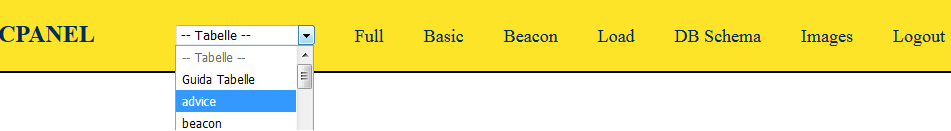
\includegraphics[width= 15cm]{navbar.png}
\end{figure} 
Per garantire una migliore esperienza di navigazione, soprattutto nella parte di amministrazione del sito; è stata inserita al top della pagina e resa fissa anche allo scroll (proprietà css \textbf{position: fixed}) una barra di navigazione (navbar). 
Come è possibile vedere dalla figura \ref{fig:navbar} la navbar è composta da vari elementi:
\begin{itemize}
\item \textbf{menù a tendina} contenente le tabelle, che è riempito dinamicamente a seconda del database selezionato;
\item \textbf{Full} : àncora che fa riferimento all'applicazione web con front-end Full (\textbf{href='full/indexp.php'});
\item \textbf{Basic} : ancora che fa riferimento all'applicazione web con front-end Basic (\textbf{href='basic/indexp.php'});
\item \textbf{Logout} : àncora che fa riferimento allo script \textbf{logout.php} che disconnette l'utente cancellandone la sessione; 
\item \textbf{Images} : àncora che fa riferimento allo script \textbf{images.php} che consente di monitorare le immagini presenti nel nostro web server alla cartella images;
\item \textbf{Beacon}, \textbf{Load}, \textbf{DB Schema} : al loro click si effettua uno scroll per mostrare a schermo la sezione del documento desiderata;
\begin{lstlisting}[language=PHP]
\end{lstlisting}
\end{itemize}
\subsubsection{Scrolling delle sezioni}
Cliccando su un'opzione o sulle ancore Beacon, Load o DB Schema viene eseguita una funzione che ci permette di scrollare la pagina a tale sezione. \newline
Per fare ciò a ogni sezione, a un elemento scelto (solitamente il primo ben in vista) gli viene assegnato al suo attributo \textbf{id} un identificativo univoco preceduto dal simbolo \#, che è lo stesso identificativo assegnato alla ancora corrispondente, in modo da essere referenziato in caso di click. 
Quindi a un evento click verrà eseguita la funzione \textbf{scroll\_function(this.value)}. \newline

\begin{lstlisting}[language=Java]
function scroll_function(string)
{
	var id = "#"+string;
	var element = document.getElementById(id);
	element.scrollIntoView();
	window.scrollBy(0,-100)
}
\end{lstlisting}
È da notare che alla funzione \textbf{window.scroll} come secondo parametro viene passato \textbf{-100}. Questo perchè la navbar ha come proprietà css \textbf{margin-top: 100px} e questo margine top viene aggiunto in modo da prevenire il \textbf{content overlay}.

\subsubsection{Sezione inserimento beacon}
Cliccando sulla ancora \textbf{Beacon} della navbar (o in alternativa scorrendo manualmente la pagina fino a tale sezione) si visualizzerà  questa sezione dedicata all'inserimento del beacon sulla mappa. \newline
Il funzionamento è facile ed intuitivo, ed è schematizzabile seguendo i seguenti passagi:
\begin{enumerate}
\item è presente la mappa di leaflet e grazie allo script \textbf{fill\_manage\_map.php} anche in questa mappa sono visibili le geometrie dei place e i beacon;
\item dopo aver scelto la posizione del nuovo beacon sulla mappa è sufficiente eseguire un \textbf{double click} per aggiungerlo;
\item verrà eseguito un evento che tramite dei \textbf{confirm} chiederà in input da parte dell'utente le altre informazioni inerenti al beacon, quali la descrizione (colonna \textit{information}), l'\textbf{id} dell'immagine custom e dell'immagine ombra custom. L'id delle due immagini possono anche essere \textbf{null}, così facendo verranno utilizzate le immagini di default;
\item se le informazioni sono state immesse correttamente e non si è scelto alcun cancel ai vari prompt mostrati, si procede all'esecuzione della query;
\item infine se la query ha dato esito negativo verrà mostrato l'errore, altrimenti si effettuerà uno scroll in un'altra sezione della pagina mostrando il beacon appena aggiunto, in una tabella;
\end{enumerate}
Di seguito il codice utilizzato per realizzare quanto detto sopra.
\begin{lstlisting}[language=PHP]
map.on('dblclick', function(e){
var lat = e.latlng.lat; 
var lng = e.latlng.lng;
var information = prompt('Inserisci le informazioni di questo beacon.');
var icon = prompt('Inserisci l\'ID dell\'icona.');
var shadow_icon = prompt('Inserisci l\'ID della shadow icon.');

var values = 'NULL,';
if(information==null || information ==='')
	values += 'NULL,';
else
	values += '\''+information +'\',';
	values += '\'' + lat + '\',\'' + lng + '\'';
if(icon ==null || icon ==='')
	values += ',NULL';
else
	values += ',\'' + icon  + '\'';        
if(shadow_icon ==null || shadow_icon ==='')
	values += ',NULL';
else
	values += ',\'' + shadow_icon  + '\'';      
document.location =   'add.php?table=beacon&values='+values;
\end{lstlisting}
\newpage
\subsubsection{Sezione Caricamento Immagini}
Cliccando sull'ancora \textbf{Load} della navbar si visualizzerà la sezione della pagina dedicata al caricamento di contenuti multimediali nella cartella \textbf{images}. 

\begin{figure}[h]
	\centering
	\label{fig:upload}
	
\includegraphics[]{upload.png}
\end{figure} 

Per caricare un'immagine si eeguono i semplici passaggi:
\begin{enumerate}
\item si clicca sul bottone \textbf{Browse} per selezionare il file dal dispositivo. Questo elemento è un input tag con attributo \textbf{type=file} definito dall'HTML5;
\item si lascia una descrizione dell'immagine che si vuole caricare nella casella di testo corrispondente;
\item infine per procedere alla richiesta caricamento effettivo basta cliccare il botton \textbf{Carica File};
\item al click del bottone si verifica che gli input file e text siano stati riempiti correttamente. In caso negativo viene mostrato un messaggio d'errore, altrimenti si esegue lo script \textit{upload.php} che effettua tutte le verifiche del caso per poi procedere al caricamento;
\end{enumerate}

\subsubsection{Database data management}
È possibile accedere a questa sezione o scrollando la pagina fino al suo inizio o selezionando una tabella del database dal menù a tendina della navbar.
Per ogni tabella del database si effettuano i medesimi passaggi.
La logica utilizzata è la seguente:
\begin{enumerate}
\item si ricava la lista delle tabelle del database selezionato (il database viene settato nel file \textit{config.php}) utilizzando l'istruzione SQL \textbf{show tables};
\item effettuata la query, tramite la funzione \textbf{mysqli\_num\_rows} si entra in un ciclo che itera quante volte quante tabelle si hanno;
\item si aggiunge dinamicamente il nome della tabella al menù a tendina;
\item si genera un tag \textbf{h1} contenente il nome di tale tabella. Oltre alla label associata, si associa al click l'evento \textbf{rename\_table} e inoltre gli viene assegnato come id, la sua label preceduta dal \# per essere referenziata per lo scrolling; 
\item viene generata un tag \textbf{table} che conterrà i dati di tale tabella; 
\item tramite il comando SQL \textbf{show columns from nome\_tabella} si ricavano tutte le colonne della tabella iterata;
\item si crea la prima riga della \textbf{table} aprendo il tag \textbf{tr};
\item effettuata la query, tramite la funzione \textbf{mysqli\_num\_rows} si entra in un altro ciclo che itera quante volte quante colonne si hanno;
\item per ogni colonna si ottengono le seguenti informazioni dall'array associativo:
\begin{itemize}
\item \textbf{Field} : Il nome della colonna;
\item \textbf{Key} : Se è un tipo di chiave particolare (primary,fk,unique,ecc..);
\item \textbf{Type} : Il tipo della colonna;
\item \textbf{Null} : Se la colonna può essere null;
\end{itemize}
\item Nell'iterazione del ciclo verranno create tante colonne (\textbf{th}) alla \textbf{table}, quante colonne ha la tabella. Quindi si apre il tag \textbf{th} e il tag \textbf{a};
\item Ogni colonna (tag \textbf{th}) ha al suo interno un'ancora (tag \textbf{a}). Vengono associati due eventi al click, uno per ciascun tag:
\begin{itemize}
\item \textbf{th} : Si chiama la funzione \textbf{change\_column};
\item \textbf{a} : Si chiama la funzione \textbf{rename\_column};
\end{itemize}
È importante dire che al trigger dell'evento click dell'elmento più interno successivamente verrà eseguito il trigger del click anche al contenitore (\textbf{bubbling}). Per prevenire ciò al click dell'elemento più interno al contenitore (in questo caso l'ancora) viene eseguita la funzione \textbf{event.stopPropagation()} per prevenire il bubbling.
\item Si verifica se null ha valore 'no'. In caso segativo si passa la punto successivo, altrimenti si apre il tag \textbf{u} (underline);
\item Si verifica se la chiave è un tipo particolare. In caso positivo si apre il tag \textbf{font} specificando una data classe definita nei fogli di stile. Dopodiché si stampa il nome della colonna e si chiude il tag. Possono verificarsi i seguenti casi:
\begin{itemize}
\item Foreign Key : il tag font avrà class='fk'; 
\begin{lstlisting}[language=PHP]
color : rgb(76, 160, 199);
\end{lstlisting}
\item Primary Key : il tag font avrà class='pk'; 
\begin{lstlisting}[language=PHP]
color : red;
\end{lstlisting}
\item Unique Key : il tag font avrà class='uq'; 
\begin{lstlisting}[language=PHP]
color : rgb(145, 120, 204);
\end{lstlisting}
\item La chiave non è un tipo particolare: quindi  non si utilizzerà nessun font tag.
\end{itemize}
\item Si verifica nuovamente se null ha valore 'no', in modo da chiudere il tag se è stato precedentemente aperto;
\item Vengono chiusi ordinatamente prima il tag dell'ancora e poi il tag dell'header della colonna;
\item Si costruisce la query \textbf{select * from nome\_tabella\_iterata} per ottenere tutti i record presenti in tale tabela;
\item Viene eseguita la query e con la funzione \textbf{mysqli\_num\_rows} si contano i record della tabella;
\item Si entra in un ciclo che itera quante volte quanti record ci sono;
\item Per ogni record si ottiene sia il nome che il valore della chiave primaria. Per i valori delle chiavi primarie si utilizza la query:
\begin{lstlisting}[language=PHP]
$primary_key_sql = "SHOW KEYS FROM ".$nome_tabella." WHERE Key_name = 'PRIMARY'";
\end{lstlisting}
\item Per ogni record si entra in un altro ciclo che itera quante volte quante colonne ha la tabella del record;
\item Per ogni colonna del record si apre il tag \textbf{td}, si associa al click l'evento \textbf{update}, si apre il tag \textbf{a} si stampa il valore del record della data colonna e si chiudono i tag aperti;
\item Se la tabella si chiama \textbf{visitors} alla cella della tabella non viene associato alcun evento al click;
\item Dopo aver stampato tutti i valori delle colonne del record viene inserita un'ulteriore colonna volta a eliminare il record. Dentro questa cella si trova un'immagine la quale è associato l'evento \textbf{delete\_row};
\item Finiti i record da inserire nella table si costruisce un'ultima riga per permettere l'inserimento manuale da parte dell'utente. (Se il nome della tabella è visitors si passa al punto successivo; viene eseguita l'istruzione \textbf{continue}) Per fare ciò si fanno delle verifiche sulle colonne:
\begin{itemize}
\item se è una chiave primaria \textbf{auto increment} non sarà presente alcuna textbox in quanto è al livello sql che viene assegnata la chiave primaria;
\item se la colonna è di tipo date, nella cella verrà stampato un input di tipo \textbf{date}.
\item se la colonna è di tipo enumerazione, nella cella verrà stampato un menù a tendina riempito con le possibili alternative (\textbf{select});
\item se è una chiave esterna verrà creato un menù a tendina riempito con i possibili valori. Per fare ciò viene utilizzata la query introdotta nella sezione 3.4.1.1;
\item si verifica infine se la colonna può essere \texttt{null} o meno. In caso positivo positivo viene stampata una semplice textbox (che può anche essere lasciata vuota) mentre in caso negativo gli viene associato un id che permetterà di essere gestito da degli eventi;
\end{itemize} 
Finite le colonne, se ne aggiunge una ulteriore contenente un'immagine che ha associato l'evento \textbf{add}, volto ad aggiungere il nuovo record.
\end{enumerate}
\begin{figure}[h]
	\centering
	\caption{Tabella exists\_table generata dinamicamente dalla logica appena introdotta.}
	\label{fig:manage}
	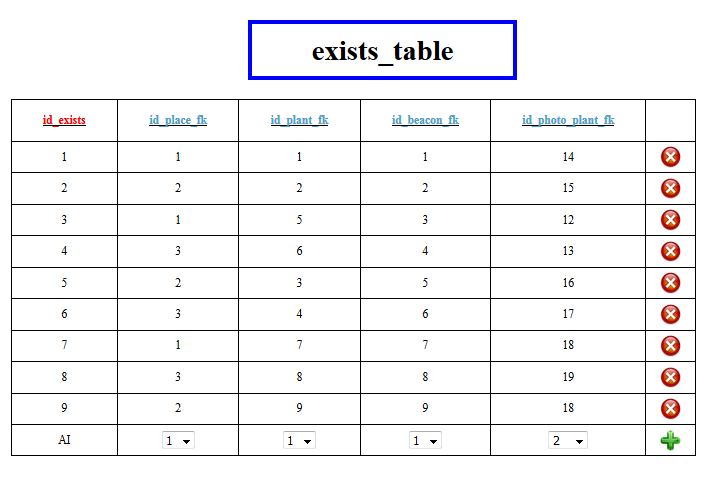
\includegraphics[width= 15cm]{manage.png}
\end{figure} 

\newpage

\subsection{Funzioni javascript impiegate nella sezione 3.3.1.5}
\subsubsection{add}
Questa funzione permette di aggiungere un nuovo record al database.
Gli vengono passati due parametri: 
\begin{itemize}
\item il nome della tabella;
\item la riga della tabella dove sono stati inseriti i valori (\textbf{tr});
\end{itemize}
Come è possibile vedere dal codice sopra, questa riga viene passata tramite l'istruzione \textbf{this.parentElement.parentElement} eseguita nel tag \textbf{img}; il parentElement di img è td e parentElement di td è tr. \newline La funzione estrapola i valori dal tag tr e li concatena con la seguente sintassi : \textit{valore1,valore2,valore3..}, nel caso la chiave primaria fosse auto incrementante la sintassi sarà la seguente: \textit{NULL,valore2,valore3..}. Ogni valore viene controllato per prevenire eventuali sequenze di escape volte a un \textbf{sql injection}.
\begin{lstlisting}[language=PHP , caption= Codice di escape]
if(element.cells[i].children[0].value.indexOf("'") > -1 || element.cells[i].children[0].value.indexOf("\"") > -1)
values = values.concat("'"+element.cells[i].children[0].value.replace(/[\\"']/g, '\\$&')+"',");   
\end{lstlisting}
Concatenati correttamente tutti i valori, dopo aver chiesto conferma all'utente, se confermato si procede al redirect come segue, invocando lo script \textbf{add.php}.
\begin{lstlisting}[language=PHP]
document.location =   "add.php?table="+table+"&values="+values;
\end{lstlisting}

\subsubsection{delete\_row}
Questa funzione consente di eliminare il record selezionato nella tabella, dal database. Vengono forniti come parametri di ingresso:
\begin{itemize}
\item il nome della tabella dal quale si vuole cancellare il record;
\item l'ancora che ha invocato questa funzione;
\item il nome della chiave primaria;
\item il valore della chiave primaria.
\end{itemize}
Dopo aver chiesto conferma dell'operazione, se confermata si procede con la seguente istruzione che permetterà il redirect alla pagina \textbf{delete.php}.
\begin{lstlisting}[language=PHP]
element.href =   "delete.php?table="+table+"&pk="+pk+"&pk_value="+pk_value;
\end{lstlisting}

\subsubsection{update}
Questa funzione consente, cliccando sulla cella che si vuole modificare, di aggiornare tale valore nel database.
Riceve i seguenti parametri di ingresso:
\begin{itemize}
\item il nome della tabella dove si trova il record da aggiornare;
\item il nome della colonna che si vorebbe aggiornare;
\item il valore che si vuole modificare;
\item il nome della chiave primaria;
\item il valore della chiave primaria.
\end{itemize}
La funzione procede come segue:
\begin{enumerate}
\item attraverso la funzione \textbf{prompt} viene chiesto il nuovo valore;
\item si verifica che il valore sia diverso da null e che ci sia stato inserito almeno un carattere, in caso negativo si esce dallo script;
\item si verifica che il valore inserito non coincida con il valore già presente nel database, in tal caso si esce dallo script mostrando la motivazione dell'errore;
\item si chiede conferma della modifica;
\item si effettue il redirect invocando lo script; \textbf{update.php} con la seguente istruzione:
\begin{lstlisting}[language=PHP]
 document.location =   "update.php?table="+table+"&new_value="+update+"&column="+column+"&pk="+pk+"&pk_value="+pk_value ;
\end{lstlisting}

\end{enumerate}

\subsubsection{rename\_column}
Questa funzione permette di rinominare una colonna di una tabella del database.
Riceve i seguenti parametri di ingresso:
\begin{itemize}
	\item il nome della tabella dove si trova la colonna da rinominare;
	\item l'ancora che ha invocato questa funzione;
	\item il nome attuale della colonna.
\end{itemize}
La funzione procede in modo analogo come la precedente.
Infine effettua il redirect invocando lo script \textbf{ rename\_c.php} come segue:

\begin{lstlisting}[language=PHP]
element.href =   "rename_c.php?column="+text+"&new_value="+update+"&table="+table ;
\end{lstlisting}

\subsubsection{rename\_table}
Questa funzione permette di rinominare una tabella.
Prende come parametro in ingresso solamente il nome attuale della tabella, che sarà confrontato con il valore inserito. Dopo aver verificato anche che il valore inserito non sia null e abbia almeno un carattere, si effettua il redirect invocando lo script \textbf{rename\_table.php} come segue:
\begin{lstlisting}[language=PHP]
document.location =   "rename_t.php?table="+table+"&new_value="+update;     
\end{lstlisting}

\subsubsection{change\_column}
Questa funzione permette di cambiare il tipo di una colonna. Gli vengono passati il nome della tabella dove si trova la colonna da modificare e il nome della colonna. \newline Dopo aver inserito il nuovo tipo, aver controllato che sia diverso da null e con un formato accettabile si chiede conferma di tale modifica.
Dopo aver confermato si effettua il redirect invocando lo script \textbf{type.php} come segue:
\begin{lstlisting}[language=PHP]
document.location =   "type.php?column="+text+"&new_value="+update+"&table="+table ;        
\end{lstlisting}
\subsection{Le differenze sostanziali tra i due front-end}
Le differenze sostanziali che intercorrono tra i due front sono schematizzabili come segue:
\begin{itemize}
\item Il FE basic è stato sviluppato in maniera \textit{old style} ossia senza seguire lo stile moderno delle applicazioni web di ultima generazione, mentre il FE full adotta stili e design di ultima generazione;
\item Il FE basic è stato stilizzato interamente con il \textbf{CSS}, senza alcun ausilio di librerie grafiche. Il FE full utilizza come framework \textbf{Materialize} che rispecchia il \textit{Material Design};
\item Il FE basic utilizza Javasript puro, mentre il FE full include la libreria di JQuery e ne fa ampio uso. (Scelta vincolante in quanto materialize inizializza i suoi componenti esclusivamente con JQuery);
\item Nel FE basic le form modali, i menù a tendina, le navbar e molti altri elementi vengono tutti gestiti manualmente tramite css e javascript. Nel FE full non ci si preoccupa di tale gestione dato che è Materialize che effettua questa parte;
\end{itemize} 
\subsection{basic front-end}
Il \textit{basic} front-end è il front end più basilare che utilizza puro codice css per essere stilizzato e puro javascript per i vari eventi.
Verranno ora analizzate alcuni aspetti legati al javascript.

\subsubsection{Menù humburgher}
Per garantire un'esperienza piacevole e intuitiva, viene utilizzato un menù richiamabile appunto dalla figura humburgher.
\begin{figure}[h]
	\centering
	\caption{Funzionamento grafico del menù}
	\label{fig:humburgher}
	
\includegraphics[width= 10cm]{humburgher.png}
\end{figure} 
Per realizzare questo effetto al click dell'humburgher non si utilizza codice javascript, ma puro CSS.
Il meccanismo si basa sul fatto che l'immagine raffigurante l'humburgher in realtà è una checkbox e la sidebar ha la proprietà transform: \textbf{translateX(-250px)}. Si gioca sulla proprietà \textbf{:checked } che al suo click permette di effettuare il translate per rendere visibile la sidebar. Per un effetto più accattivante viene settata una transizione di 250ms ease-in-out.
\newline \newline
Il menù è composto dalle seguenti voci:
\begin{itemize}
\item Effettua una ricerca : apre la finestra modale della ricerca;
\item Gestisci il database : apre la finestra modale del login;
\item Scatta una foto : apre la finestra modale per scattare foto;
\item Nascondi Beacons : nasconde i beacon dalla mappa. Al click questa voce prende la label 'Mostra beacons' che consente di effettuare l'operazione opposta;
\item Nascondi Poligoni : nasconde i poligoni dalla mappa. Al click questa voce prende la label 'Mostra poligoni' che consente di effettuare l'operazione;
\item Segnala un problema : apre la finestra modale per inviare i report;
\item Aggiorna la pagina : effettua un refresh della pagina;
\item Full website : effettua un redirect all'altro front-end. (full front-end ).
\end{itemize}

\subsubsection{Principio di funzionamento delle finestre modali}
In questo format dell'applicazione web, si fanno ampio uso delle finestre modali, che vengono richiamate tramite il menù humburgher.
Il principio di funzionamento è semplice: ogni form viene nascosta o mostrata tramite seguente istruzione javascript che modifica una proprietà css.
\begin{lstlisting}[language=PHP]
var modal = document.getElementById('myModal'); /*recupero la form dall'id*/
modal.style.display = "none"; /*nasconde la form*/
modal.style.display = "block"; /*mostra la form*/
\end{lstlisting}
Quando viene mostrata la form, viene aggiunto un overlay css con colore rgba(0,0,0,0.5).
Per chiudere la finestra è sufficiente premere l'immagine di chiusura (una x in alto a destra) o cliccare ovunque fuori la form.

\subsubsection{Finestra modale - Login}
Questa finestra modale permette di effettuare il login e accedere alla pagina \textit{manage.php}. 
\begin{figure}[h]
	\centering
	\caption{Grafica della Login Form}
	\label{fig:login}
	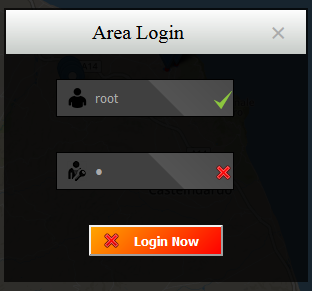
\includegraphics[]{login.png}
\end{figure} 
Come è possibile vedere dall'immagine, troviamo la x per chiudere tale form, due campi per inserire le credenziali e il bottono submit.
Ecco alcune caratteristiche degne di nota delle caselle di testo (\textbf{input} tags):
\begin{itemize}
\item ottengono tale effetto grafico tramite un gradiente lineare;
\begin{lstlisting}[language=Java]
 linear-gradient(45deg, #404040 0%, #404040 60%, #535353 60%,
#494949);
\end{lstlisting}
\item Presentano un padding tale da inserire un'icona inerente al campo.
Quest'effetto si raggiunge utilizzando la proprietà \textbf{background};
\begin{lstlisting}[language=Java]
background: url('../../images/icon.png') 10px center no-repeat, -webkit-linear-gradient(45deg, #404040 0%, #404040 60%, #535353 60%, #494949);
\end{lstlisting}
\item All'evento keyup viene associata una funzione che controlla se il testo inserito supera dei determinati controlli. (In questo caso che la lunghezza minima sia di 4 caratteri). A seconda dell'esito dei controlli viene mostrata l'immagine corrispondente. Per inserire le immagini rispettivamente con padding sia a destra che a sinistra si utilizza sempre la proprietà background che viene formattata come segue;
\begin{lstlisting}[language=Java]
background : url('../../images/icon_left.png') 10px center no-repeat, url('../../images/icon_right.png')  right 10px no-repeat , linear-gradient(45deg, #404040 0%, #404040 60%, #535353 60%, #494949);
\end{lstlisting}
\item Ad ogni evento keyup si controlla se entrambi i campi sono stati fillati correttamente. In caso positivo si abilita il bottone submit che effettua il redirect allo script \textit{login.php} procedere all'autenticazione.

\end{itemize}

\subsubsection{Finestra modale - Segnala}
Questa finestra modale permette di inviare una segnalazione e registrarla nel database. È composta da una \textbf{textarea} e un \textbf{submit}. Inoltre nella form vengono salvate le variabili che tengono traccia della posizione dell'utente, delll'accuratezza e dell'altitudine. (queste variabili vengono inizializzate dalla geolocation API se si è acconsentito alla geolocalizzazione, altirmenti sono null) \newline All'evento \textbf{onsubmit} si controlla che la segnalazione non sia vuota e si procede ad esegire lo script \textit{report.php}.

\subsubsection{Finestra modale - Scatta Foto}
Questa finestra modale permette di scattare delle foto, registrarle nel database e caricarle nella cartella \textit{images}.
Si procede come segue:
\begin{enumerate}
\item si scatta la foto premendo il bottone \textit{Scatta};
\item il canvas viene riempito con l'immagine acquisita usando la funzione \newline \textbf{canvas.getContext('2d').drawImage(...)};
\item premendo il bottone \textit{Carica} si verifica se il canvas non è vuoto (creandone uno nuovo e vuoto dinamicamente e confrontandolo);
\item attraverso la funzione \textbf{prompt} viene chiesto all'utente di inserire la descrizione della foto appena scattata, si controlla che non sia null e che abbia almeno un carattere;
\item si inoltra una richiesta \textbf{Xml Http Request} per il caricamento (analizzata successivamente).
\end{enumerate}

\subsubsection{Finestra modale - Ricerca}
Questa finestra modale permette di effettuare una ricerca tra elementi di interesse che abbiamo nella nostra mappa.
\begin{figure}[h]
	\centering
	\caption{Grafica della Form per la ricerca}
	\label{fig:search_basic}
	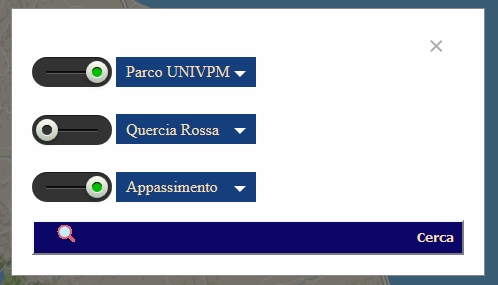
\includegraphics[scale=0.9]{search_basic.png}
\end{figure} 
I filtri desiderati si abilitano con appositi checkbox stilizzati in stile slide e si selezionano tramite menù a tendina che come detto in precedenza vengono fillati dinamicamente dal proprio script del front end \textit{fill.php}. \newline
Cliccando il bottone \textit{Cerca} si esegue la funzione \textbf{search()} che formatta l'url del redirect in base ai filtri abilitati e scelti.
Si procede nel seguente modo:
\begin{enumerate}
\item si ottengono gli elementi delle checkbox;
\item si ottengono gli elementi dei menù a tendina;
\item si verifica se i menù a tendina non sono inizializzati, ciò vuoldire che non ci sono dati sufficienti per effettuare la ricerca e lo script si interrompe mostrando il relativo messaggio d'errore;
\item si verifica se almeno un filtro di ricerca è stato abilitato, altrimenti lo script si interrompe mostrando il relativo messaggio d'errore;
\item per ogni filtro abilitato e scelto si procede alla creazione dinamica dell'url utilizzando concatenazioni di stringhe attraverso l'operatore ternario;
\end{enumerate}
Di seguito il codice utilizzato per realizzare i passaggi sopra descritti.
\begin{lstlisting}[language=PHP]
function search()
{
/*filtri abilitati*/
var place_check_var = document.getElementById('slide_place').checked;
var species_check_var = document.getElementById('slide_species').checked;
var phase_check_var = document.getElementById('slide_phase').checked;

/*filtri selezionati*/
var place_var = document.getElementById("place-select");
var species_var = document.getElementById("species-select");
var phase_var = document.getElementById("phase-select");


var name_place_selected_var = "";
var name_species_selected_var = "";
var name_phase_selected_var = "";

/*nel caso si forzasse l'apertura della modale utilizzando dei tricks*/
if((place_var.selectedIndex ==-1) && (species_var.selectedIndex ==-1) && (phase_var.selectedIndex==-1))
{
alert("Non ci sono dati nella mappa per effettuare una ricerca.");
return false;
}

/*se non sono stati selezionati filtri*/
if((place_check_var===false) && (species_check_var===false) && (phase_check_var===false))
{
alert("Seleziona almeno un filtro di ricerca.");
return false;
}

if((place_var.selectedIndex !=-1) && (place_check_var===true))
name_place_selected_var = place_var.options[place_var.selectedIndex].value;

if((species_var.selectedIndex !=-1) && (species_check_var===true))
name_species_selected_var = species_var.options[species_var.selectedIndex].value;


if((phase_var.selectedIndex!=-1) && (phase_check_var===true))
name_phase_selected_var = phase_var.options[phase_var.selectedIndex].value;

var url = "homepage.php?";
url += name_place_selected_var==""? "": "place="+name_place_selected_var;
url += (name_species_selected_var =="" ?  "" : (name_place_selected_var==""? "species="+name_species_selected_var : "&species="+name_species_selected_var));
url += (name_phase_selected_var ==""? "" : ((name_place_selected_var=="" && name_species_selected_var =="")? "phase="+name_phase_selected_var : "&phase="+name_phase_selected_var));

console.log(url); /*si rgistra nella console l'url di ricerca*/
window.location.href = url;
}
\end{lstlisting}
Esempio di url generato in caso di ricerca secondo i filtri scelti e abilitati dell'immagine \ref{fig:search_basic} : \newline
\newline \textbf{homepage.php?place=3\&phase=Appassimento} \newline \newline
Come precedentemente introdotto, dopo aver effettuato il redirect, nella pagina homepage si verificano se sono stati passati dei parametri. Essendo stati passati i parametri place e phase si eseguirà lo script \textit{search.php}.

\subsubsection{Finestra Modale dei beacon - Funzione create\_popup(..)}
Al click di ogni beacon (pianta) presente sulla mappa viene associato l'evento \textbf{create\_popup}. Questo evento è volto a creare dinamicamente una form modale contenente tutte le informazioni del beacon cliccato e mostrarla a schermo. Di seguito un esempio della form:
\begin{figure}[h]
	\centering
	\label{fig:create_popup}
	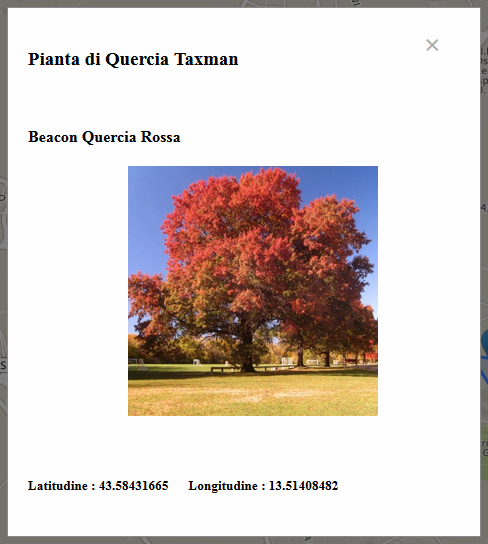
\includegraphics[scale=0.8]{create_popup.png}
\end{figure} 
\newline
Come è possibile vedere dalla foto, la form è formata dalle seguenti parti, partendo dall'alto:
\begin{itemize}
\item il tag \textbf{h3} che conterrà il nome della pianta dove è stato posizionato il beacon;
\item il tag \textbf{h4} che conterrà le informazioni del beacon; 
\item il tag \textbf{img} rappresentante l'immagine della pianta; 
\item due tag \textbf{h5} rappresentanti rispettivamente uno la latitudine e l'altro la longitudine del beacon.
\end{itemize}
Per far si che ogni beacon (pianta) sulla mappa abbia una propria form contenente i propri dati si è scelto di utilizzare una singola form dove ad ogni click vengono modificati dinamicamente tutti i tag introdotti sopra.  dalla funzione associata al beacon. La modifica viene fatta dalla funzione che si sta analizzando.
Per capire il funzionamento andremo ad analizzare il codice di quest'ultima.
\newline
Dalla form risulta facile capire quali sono i parametri che gli vengono passati a questa funzione:
\begin{itemize}
\item il nome della pianta. (colonna \textit{name\_plant} della tabella \textit{plant});
\item le informazioni del beacon. (colonna \textit{information} della tabella \textit{beacon});
\item il path della foto della pianta. (\textit{id\_photo\_plant\_fk} della tabella \textit{exists\_table});
\item la latitudine e la longitudine del beacon. (colonne \textit{lat} e \textit{lng} della tabella \textit{beacon}).
\end{itemize}
Si ricorda che questi parametri vengono passati dinamicamente dallo script che inizializza la mappa. (\textit{init.php})
\newline
Si effettuano i seguenti controlli sulle variabili passate:
\begin{itemize}
\item  si verifica se il path dell'immagine è null: in tal caso non si ha nessuna immagine per la pianta e viene messa un'immagine di default;
\item si verifica se si hanno informazioni sul beacon (la colonna information può anche essere null). In caso negativo si stampa un'etichetta che esprime tale mancanza;
\item si verifica che il nome della pianta sia diverso da null : se fosse null il beacon non è associato dal alcuna pianta. In questo caso viene mostrata la label dedicata (beacon non associato) e viene messa un'immagine di default.
\end{itemize}
Quanto detto sopra è riassumibile nel codice utilizzato.

\begin{lstlisting}[language=PHP]
function create_popup(plant_name,information,path,lat,lng)
{ 

if(path == '' || path == null || path =='null' || path === 'null')
document.getElementById('plant_photo').src = "../images/no-image.jpg";

else
document.getElementById('plant_photo').src = "../images/"+path;

if(information == 0 || information == null || information === null || information =='null' || information ==='null')
document.getElementById('beacon_info').innerHTML = "Nessuna informazione per questo beacon";
else
document.getElementById('beacon_info').innerHTML = information;

if(plant_name == 0 || plant_name == null || plant_name === null || plant_name =='null' || plant_name ==='null')
document.getElementById('plant_name').innerHTML = "Beacon non associato";
else
document.getElementById('plant_name').innerHTML =plant_name;


document.getElementById('beacon_lat').innerHTML = "Latitudine : "+lat;
document.getElementById('beacon_lng').innerHTML = "Longitudine : "+lng;

beacon_modal();
}
\end{lstlisting}
\subsubsection{Caricamento del Canvas con Xml HTTP Request}
Al click del bottone \textit{Carica} della form per scattare una foto, si chiama la funzione \textbf{load\_canvas}.
Questa funzione invia una richiesta \textbf{XHR} per caricare asincronamente il contenuto multimediale. Il funzionamento può essere riassunto dicendo semplicemente che viene creata una \textbf{Form Data} contenente i dati che si vogliono mandare al server in modo asincrono e con la funzione \textbf{send} si inviano tali dati.
\newline Il codice utilizzato per la XHR è il seguente:
\begin{lstlisting}[language=PHP]
var dataURL = canvas.toDataURL("image/png");
document.getElementById('hidden_data').value = dataURL;
var fd = new FormData(document.forms["form1"]);

var xhr = new XMLHttpRequest();
xhr.open('POST', '../php/upload_canvas.php', true);

xhr.upload.onloadend = function(e) {
	alert('Upload eseguito con successo.');
};
xhr.send(fd);
\end{lstlisting}

\newpage
\subsection{Full Front-End}

Il \textit{full} front-end è il front-end con funzioni più eleganti, sia dal punto di vista grafico che dal punto di vista del codice. \newline Come già detto, tutti gli eventi e stili sui vari elementi utilizzati (form modali, menù a tendina ecc..) vengono gestiti dal framework. Verranno analizzati alcune funzionalità grafiche e funzionali del JQuery mentre non verranno nuovamente affrontate construtti o form che risultino strutturalmente identiche a quelle dell'altro front-end.
\subsubsection{Side Navbar}
Come per l'altro front-end, anche in questo viene inserita una sidebar sulla sinistra. Quasi tutte le funzioni e le ancore sono le stesse, ad eccezione di come si effettua la ricerca che verrà analizzata successivamente.  \newline
In questa barra troviamo una particolare funzionalità del framework grafico, la \textbf{Collapsible} che è una sorta di menù a tendina collassabile che si espande al click.
La voce Segnala un problema non è presente nella sidebar ma è stata posizionata sulla navbar, esattamente in alto a destra. \newline
La sidebar è composta dalle seguenti voci:
\begin{itemize}
\item \textbf{Effettua la ricerca} : Ancora che permette di effettuare la ricerca invocando lo \textit{script.php};
\item \textbf{Place} : è un Collapsible "fillato" dinamicamente con tutti gli orti botanici memorizzati nel sistema;
\item \textbf{Species} : è un Collapsible fillato dinamicamente con tutte le specie memorizzate nel sistema;
\item \textbf{Phenological} Phase : è un Collapsible fillato dinamicamente con tutte le fasi fenologiche memorizzate nel sistema;
\item \textbf{Filtri} : è un Collapsible dove all'interno è possibile visualizzare i filtri scelti e resettarli;
\item \textbf{Scatta una Foto} : ancora che permette di aprire la finestra modale relativa al caricamento di contenuti multimediali;
\item \textbf{Nascondi Beacons }: ancora che permette di nascondere tutti i beacon dalla mappa. Al click quest'ancora prende la label 'Mostra Beacons' che consente di effettuare l'operazione opposta;
\item \textbf{Nascondi Poligoni} :ancora che permette di nascondere tutti gli orti botanici dalla mappa. Al click quest'ancora prende la label 'Mostra Poligoni' che consente di effettuare l'operazione opposta;
\item \textbf{Gestisci il Database} : ancora che permette di aprire la finestra modale relativa all'inserimento delle credenziali per effettuare il login ed accedere a \textit{manage.php};
\item \textbf{Aggiorna la Pagina} : ancora che effettua il refresh della pagina;
\item \textbf{Basic Website} : ancora che effettua un redirect all'altro front-end (basic front-end).
\end{itemize}

\subsubsection{Form Caricamento Immagini}
La parte di WebRTC non viene utilizzata, per gestire la fotocamera si usa il tag input dell'\textbf{HTML5} di tipo file. Questo tag si comporta in modo differente a seconda del dispositivo:
\begin{itemize}
\item In una piattaforma desktop si aprirà la \textbf{file browser dialog} che permetterà di caricare un file esistente;
\item In una piattaforma mobile (smartphone) si aprirà la fotocamera con l'applicazione di sistema : dopo aver scattato la foto il dispositivo chiederà di utilizzarla o meno, assegnandola all'elemento html.
\end{itemize} 
Ecco come si presenta la form : 

\begin{figure}[h]
	\centering
	\label{fig:upload_full}
	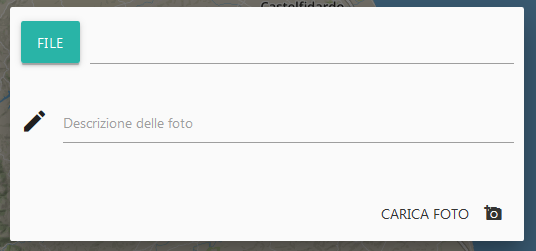
\includegraphics[]{upload_full.png}
\end{figure} 
Effettuando il click su \textit{Carica Foto}, dopo aver superato i controlli di validità sui dati, si esegue come per il caricamento del canvas, un richiesta asincrona.
Anche qui si crea una \textbf{Form Data} dove si appendono i dati da inviare in modo asincrono al server.
La richiesta viene effettuata con il JQuery:
\begin{lstlisting}[language=PHP]
var file_data = $('#fileToUpload').prop('files')[0];   
var descr_data = $('#descr_text').val();   
var form_data = new FormData();                  
form_data.append('file', file_data); 
form_data.append('descr_text',descr_data);                    
$.ajax({
	url: 'php/upload.php', 
	dataType: 'text',  
	cache: false,
	contentType: false,
	processData: false,
	data: form_data,                         
	type: 'post',
	success: function(){
		var upload_success = "<span>Upload Eseguito con successo.</span>";
		M.toast({html: upload_success,classes: 'rounded'});
	},
	error: function(xhr){
		var error = '<span> Request Status: ' + xhr.status + ' Status Text: ' + xhr.statusText + ' ' + xhr.responseText +'</span>'
		M.toast({html: error});  
	}
});
\end{lstlisting}
Appena la richiesta asincrona è conclusa, viene mostrato un messaggio attraverso la funzionalità \textbf{Toast} di Materialize.
Ecco un esempio in caso di caricamento eseguito con successo:

\begin{figure}[h]
	\centering
	\label{fig:upload_success}
	
\includegraphics[]{upload_success.png}
\end{figure} 

\subsubsection{Effettuare una Ricerca}
In questo front-end la ricerca ha come obiettivo di essere espletata con meno interazioni possibili da parte dell'utente. Non viene quindi utilizzata una form ma i \textbf{Collapsible} della sidebar.\newline
Per effettuare una ricerca si procede come segue:
\begin{enumerate}
\item si effettua un click sul Collapsible del filtro desiderato;
\item si sceglie il filtro desiderato dal Collapsible che si è espanso;
\item al click del filtro scelto verrà eseguito un Toast con la scelta effettuata;
\item si procede alla scelta o meno degli altri filtri;
\item per visualizzare i filtri immessi o resettarli basta navigare tra gli elementi del Collapsible \textbf{Filtri};
\item infine basta cliccare su \textbf{Effettua La Ricerca}.
\end{enumerate}
L'url creato dinamicamente con i filtri selezionati viene creato in modo analogo a quello dell'altro front-end.
Appena viene effettuata la ricerca, si esegue un \textbf{Toast} con il suo esito.

\begin{figure}[h]
	\centering
	\label{fig:search_toast}
	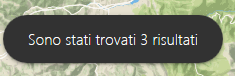
\includegraphics[]{search_toast.png}
\end{figure} 

\subsubsection{Finestra Modale dei beacon - Funzione create\_popup(..)}
Anche in questo front-end le finestre modali vengono create con la stessa identica logica analizzata nella sezione \textbf{3.3.4.7}. A differenza dell'altro front-end in questo grazie a Materialize, oltre a un design più accattivante viene utilizzata \textbf{Material Box} che è un'implementazione del del plugin material design \textbf{Lightbox}. Al click dell'immagine Material Box la centra e la allarga con un dolce effetto di transizione. Per uscire dall'immagine ingrandita è sufficiente premere ESC, cliccare sull'immagine o scrollare la pagina.


\subsection{Javascript vs JQuery}

\subsubsection{Approccio nel Coding}
Si può affermare che usando 
\begin{lstlisting}[language=PHP]
$('#myElement').click(function(){ ... });	/*JQuery*/
\end{lstlisting}
sia meglio dal punto di vista dell'\textbf{event registration model} dato che JQuery usa internamente \textbf{addEventListener} and \textbf{attachEvent} per gestire gli eventi. \newline
Registrando  un evento utilizzando questa scrittura moderna è un modo di gestire gli eventi con \textbf{Unobtrusive JavaScript}. \newline
L' Unobtrusive JavaScript è un tipo di approccio che prevede che:
\begin{itemize}
\item separazione delle funzionalità (\textit{behavior layer}) della struttura/contenuto e presentazione della pagina web;
\item migliori pratiche per evitare i problemi della programmazione JavaScript tradizionale (come le incoerenze del browser e la mancanza di scalabilità);
\item miglioramento progressivo per supportare i programmi utente che potrebbero non supportare la funzionalità JavaScript avanzata.
\end{itemize}
Inoltre per registrare più di un event liestener per un target si può chiamare addEventListener() per lo stesso target come segue:
\begin{lstlisting}[language=PHP]
var myEl = document.getElementById('myelement');

myEl.addEventListener('click', function() {
alert('Ciao Mondo!');
}, false);

myEl.addEventListener('click', function() {
alert('Ciao Mondo di nuovo!');
}, false);
\end{lstlisting}

Altri metodi come l'\textbf{HTML attributes}:
\begin{lstlisting}[language=PHP]
<button onclick="alert('Ciao Mondo!')">
\end{lstlisting}
oppure come il \textbf{DOM element properties}:
\begin{lstlisting}[language=PHP]
myEl.onclick = function(event){alert('Ciao Mondo');}; 
\end{lstlisting}

sono vecchi paradigmi e possono essere sovrascritti facilmente, questo perchè :

\begin{itemize}
\item l'attributo HTML dovrebbe essere evitato in quanto rende il markup più grande e meno leggibile. Struttura / contenuto e comportamento non sono ben separate, rendendo più difficile trovare un bug;

\item il problema con il metodo delle proprietà dell'elemento DOM (Document Object Model) è che solo un gestore di eventi può essere associato a un elemento per evento.
\end{itemize}

\subsubsection{Performance}
Per una migliore performance si usa il JavaScript nativo mentre per uno sviluppo più veloce si usa jQuery. \newline

Effettuando un test con Firefox 16.0 32-bit su Windows Server 2008 R2 / 7 64-bit sulla performance si ottengono i seguenti dati:


\begin{lstlisting}[language=PHP]
$('myElement'); /*6,604 operations per second - JQuery*/
document.getElementsByTagName('myElement'); /*10,331,708 operations/sec - Native Javascript*/
\end{lstlisting}

 \clearemptydoublepage
\chapter{Set up dell'applicazione web}
In questo capitolo vengono introdotti i software che permetteranno di configurare  l'applicazione web realizzata affinché sia online.

\section{Hosting}
L'hosting è un servizio che permetta di caricare dei contenuti su un server web affinché sia accessibile dalla rete internet.
Si utilizza un Hosting di Amazon (a pagamento) che è una macchina virtuale dove vi è installato \textbf{Bitnami} (web server), e vi tutti gli strumenti necessari per procedere al setup.

\section{Database}
Si procede alla creazione del database sul nostro host, è necessario quindi connettersi al modulo PhpMyAdmin dell'hosting.

\subsection{Putty Setup}
Per effettuare il setup dell'applicativo Putty si devono effettuare i seguenti passaggi:
\begin{enumerate}
\item installare il Client SSH per la gestione in remoto di sistemi informatici \textbf{Putty};
\item aprire Putty;
\item nella sezione \textbf{Session}, nel campo \textbf{Host Name} inserire l'indirizzo IP del nostro hosting;
\item selezionare la porta 80;
\item entrare sezione \textbf{Connection};
\item entrare nella sotto sezione \textbf{SSH};
\item selezionare la voce \textbf{Auth};
\item nella sezione \textbf{Authentication Parameters} trovare la voce \textbf{Private key File for Authentication}, cliccare Sfoglia/Browse e selezionare il file di autenticazione fornitoci (\textit{LightEC2private.ppk});
\item sempre nella sotto sezione SSH selezionare la voce \textbf{Tunnels};
\item settare la \textbf{Source Port} con \textbf{8888};
\item settare \textbf{Destination};
\item cliccare Aggiungi/Add;
\item assicurarsi che la porta aggiunta sia tra le \textbf{Forwarded Ports};
\item cliccare \textbf{Apri/Open} per aprire la connessione SSH con il server. La sessione SSH includerà ora un tunnel SSH sicuro tra le due porte specificate;
\item inserire come username \textbf{bitnami};
\end{enumerate}

\begin{figure}[h]
	\centering
	\caption{Connessione stabilita con successo}
	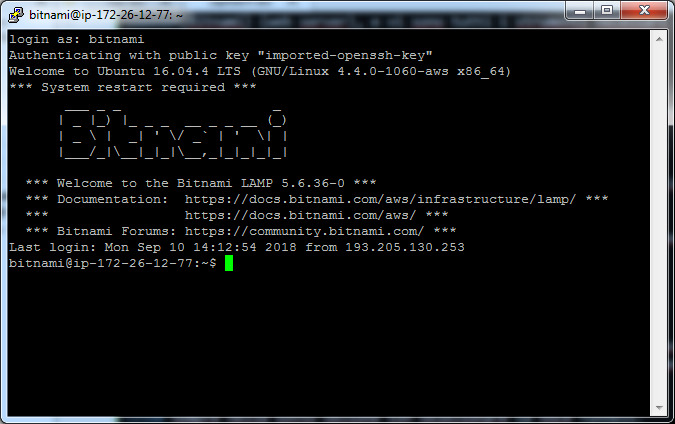
\includegraphics[width= 15cm]{bitnami.png}
\end{figure}
Lasciando il terminale aperto si prosegue con la connessione a phpmyadmin.
\subsubsection{Connessione a PhpMyAdmin}
Per connettersi a questo modulo si procede come segue:
\begin{enumerate}
\item si apre il web browser;
\item si naviga all'indirizzo \textbf{http://127.0.0.1:8888/phpmyadmin/};
\item si apre il pannello di login di phpmyadmin come in figura:
\begin{figure}[h]
	\centering
	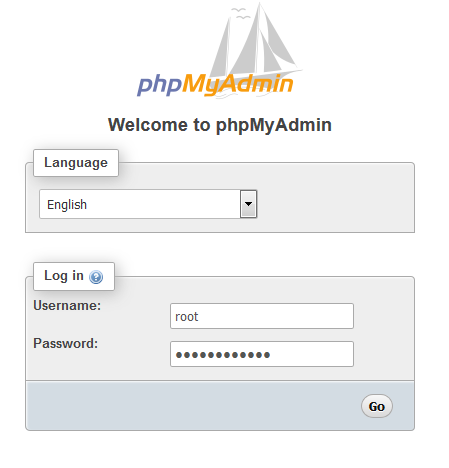
\includegraphics[width= 13cm]{phpmyadmin.png}
\end{figure}


\item si immettono le credenziali - Username : \textbf{root} -Password;
\item si clicca \textbf{Go} per entrare nel pannello di PhpMyAdmin;
\end{enumerate}
\newpage
Entrati nel pannello si procede alla creazione del database, cliccando sulla voce new dalla \textbf{tree-view} sulla sinistra. Fare riferimento alla seguente immagine.
\begin{figure}[h]
	\centering
	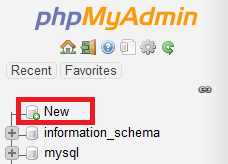
\includegraphics[]{create_database.png}
\end{figure}

Ora si procede come segue:
\begin{enumerate}
\item Inserire il nome del database (\textbf{orto\_botanico}).
\item Selezionare il set di caratteri \textbf{utf8\_general\_ci}.
\item Premere il bottone \textbf{Create}.
\item Selezionare dalla tree-view il database \textbf{orto\_botanico}.
\item Cliccare la Tab \textbf{SQL}.
\item Creare le tabelle definite una per una nella sezione \textbf{3.1.3}. Le tabelle devono rispettare il seguente ordine a causa delle dipendenze da chiavi esterne:
\begin{itemize}
\item \textbf{photo};
\item \textbf{beacon};
\item \textbf{species};
\item \textbf{phenological\_phase};
\item \textbf{place};
\item \textbf{plant};
\item \textbf{exists\_table};
\item \textbf{visitors};
\item \textbf{advice};
\end{itemize}
\end{enumerate}
A questo punto è possibile iniziare a inserire i dati nel database. 
\newpage
\subsection{geojson.io}
Per comodità per la \textbf{latitudine} e \textbf{longitudine} di un elemento e per il \textbf{boundary} di un orto botanico si utilizza il sito web \textbf{http://geojson.io}. Ecco un esempio di utilizzo:

\begin{figure}[h]
	\centering
	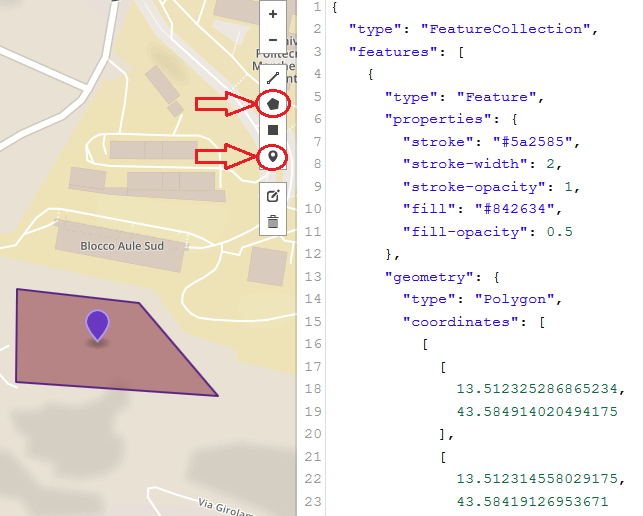
\includegraphics[scale=0.9]{geojson.png}
\end{figure}

Come è possibile vedere dall'immagine, sulla destra troviamo il codice che poi sarà inserito nella colonna \textbf{boundary}. Sul riquadro della mappa invece, sulla destra si trova una sidebar volta a creare vari elementi. Quelli cerchiati sono quelli di interesse, utilizzati nel progetto. \newline 
Inoltre cliccando sull'elemento creato nella mappa è possibile specificare ulteriori parametri come suggeriscono le seguenti immagini.

\begin{figure}[H]
	\centering
	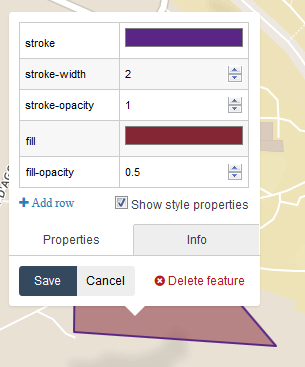
\includegraphics[]{place1.png}
	\caption{Click sul poligono : possibilità di specificare attributi grafici come il colore, la linea di contorno e l'opacità.}
\end{figure}

\begin{figure}[H]
	\centering
	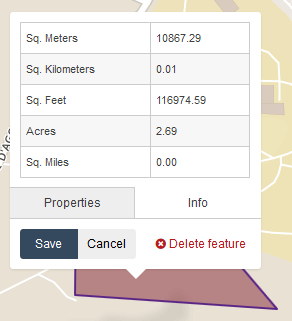
\includegraphics[]{place2.png}
	\caption{Click sul poligono : informazioni utili.}
\end{figure}

\begin{figure}[H]
	\centering
	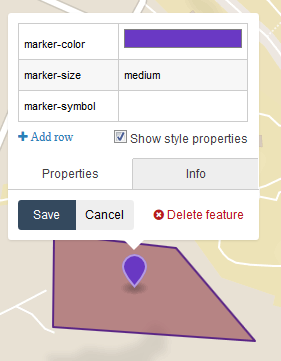
\includegraphics[]{beacon1.png}
	\caption{Click sul beacon : possibilità di specificare attributi grafici come il colore, il simbolo e la dimensione.}
\end{figure}

\begin{figure}[H]
	\centering
	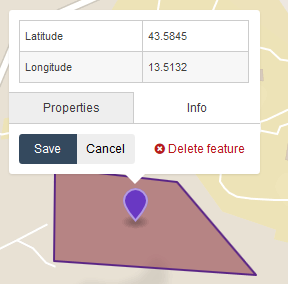
\includegraphics[]{beacon2.png}
	\caption{Click sul beacon : latitudine e longitudine.}
\end{figure}

\section{Caricamento Files con WinSCP}
WinSCP, acronimo di Windows Secure Copy che è un client SFTP e FTP di tipo grafico che ha come funzione principale quella di trasferimento dati tra un computer locale ed uno remoto. In più WinSCP consente semplici funzionalità di file manager. Per trasferimenti sicuri usa Secure Shell (SSH) e supporta il protocollo SCP in aggiunta al SFTP \cite{sito_winscp}.  \newline
Per configurare la connessione e effettuare il caricamento dei file si procede come segue:
\begin{enumerate}
\item si Installa WinSCP;
\item si avvia il client WinSCRP;
\item si imposta l'indirizzo IP;
\item si imposta come username \textbf{bitnami};
\item si clicca su \textbf{Advanced}, a questo punto si apre una finestra;
\item cliccare la sezione \textbf{SSH};
\item aprire la voce \textbf{Authentication};
\item immettere la chiave \textit{LightEC2private.ppk} sul campo \textbf{Private Key File};
\item sfogliare le directory del server fino a raggiungere \textbf{/opt/bitnami/apache2/htdocs};
\item trascinare i files desiderati ricordando di applicare le modifiche al file config.php che sviluppando in locale ha parametri differenti;
\end{enumerate}

\section{Disabilitare il modulo Pagespeed}
Per evitare eventuali problemi di visualizzazione delle icone dei beacon sulla mappa, è necessario disabilitare il modulo pagespeed.
Per fare ciò bisogna localizzare il file \textbf{pagespeed.conf} che è situato nella directory \textbf{/opt/bitnami/apache2/conf}, aprire il file e modificare la linea \textbf{ModPagespeed on} in \textbf{ModPagespeed off}. 
Infine è necessario riavviare il servizio di apache con il comando \textbf{service httpd restart}.


\newpage

\section{Permessi per uploads}
Per far funzionare correttamente gli script php di upload e non incorrerre errori particolari è necessario dare tutti i permessi alle seguenti cartelle:
\begin{itemize}
\item /opt/bitnami/php/tmp
\item /opt/bitnami/apache2/htdocs/images
\end{itemize}
Questa operazione può essere effettuata tramite terminale con i seguenti passaggi:
\begin{enumerate}
\item Ci si assicura che la connessione SSH sia aperta.
\item Si ottengono i permessi di amministratore utilizzando il comando \textbf{sudo su}.
\item Si esegue l'istruzione chmod 755 -R /opt/bitnami/php/tmp per i permessi della cartella temp.
\item Si esegue l'istruzione chmod 755 -R /opt/bitnami/apache2/htdocs/images per i permessi della cartella images.
\end{enumerate}
In alternativa è possibile utilizzare \textbf{WinSCP} : cliccando su proprietà è possibile impostare i permessi come in figura.
\begin{figure}[H]
	\centering
	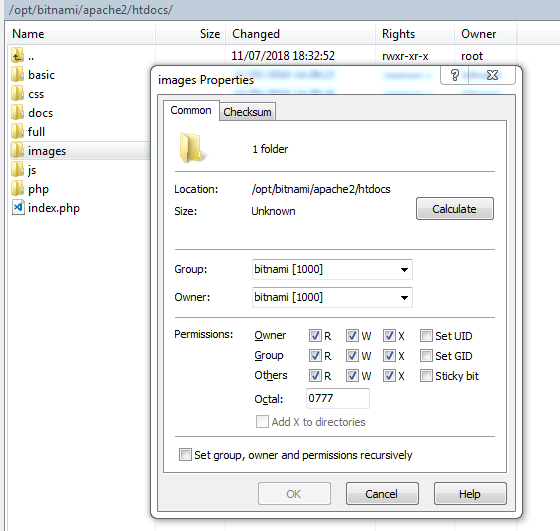
\includegraphics[scale=0.7]{permission.png}
	\caption{Proprietà : Assicurarsi che Write sia spuntato}
\end{figure}

\section{Accesso all'applicazione Web con il protocollo HTTPS}
Per accedere da desktop all'applicazione web utilizzando il protocollo sicuro è necessario aggiungere un'eccezione al certificato che è \textbf{self-signed}. \newline
\begin{figure}[H]
	\centering
	\caption{Aggiungendo l'eccezione è possibile navigare nel sito utilizzando a pieno le API}
	\label{fig:firefox_https}
	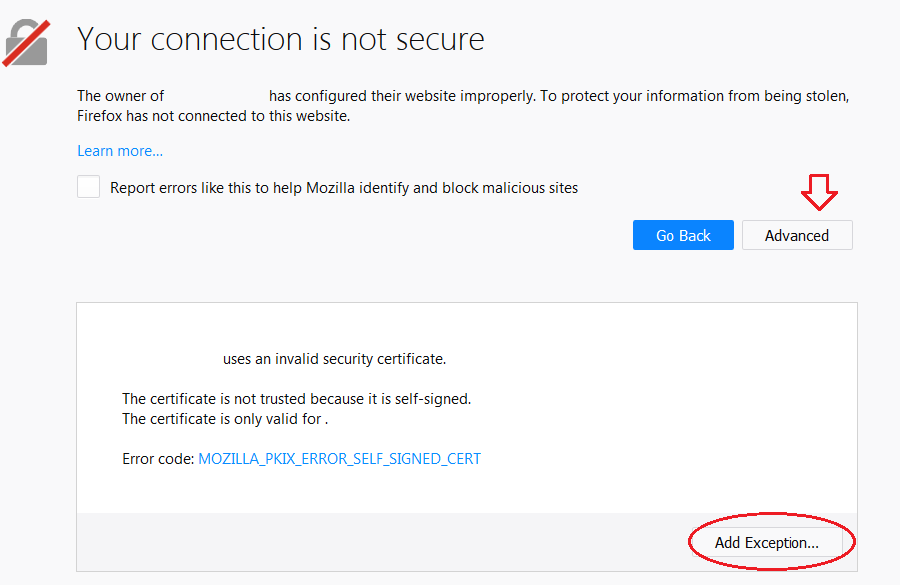
\includegraphics[scale=0.6]{firefox_https.png}
\end{figure} 

\begin{figure}[H]
	\centering
	\caption{Confermando l'eccezione sarà possibile la navigazione}
	\label{fig:exception}
	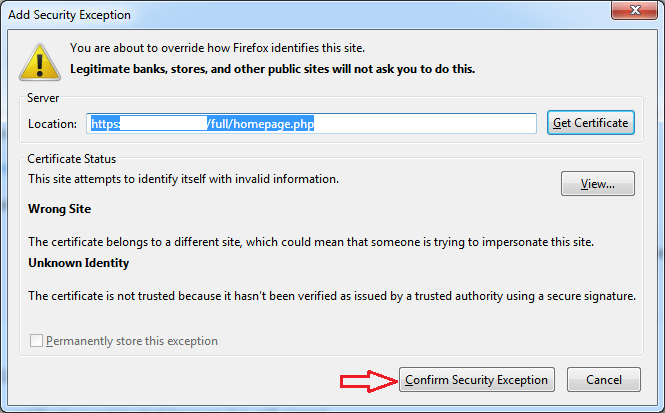
\includegraphics[scale=0.6]{exception.png}
\end{figure} 

\begin{figure}[H]
	\centering
	\caption{Richiesta di Localizzazione da Desktop}
	\label{fig:geolocation_desktop}
	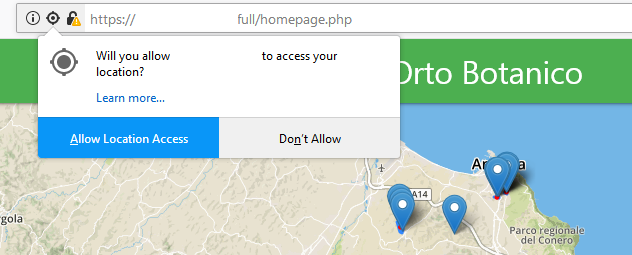
\includegraphics[scale=0.6]{geolocation_desktop.png}
\end{figure} 

\newpage

\section{Gestione del Database tramite script manage.php}
Dopo aver eseguito tutte le configurazioni precedentemente introdotte, tramite la pagina manage.php non si ha più necessità di utilizzare il modulo PhpMyAdmin per manipolare i dati nel database. \newline
Ora verranno introdotte le funzioni restanti messe a disposizione da questo script che non sono state introdotte in precedenza.
\begin{itemize}
\item modifica del nome di una tabella, cliccando semplicemente sul nome;
\item notifica tooltip del tipo della colonna, lasciando il puntatore (evento \textbf{onhover}) sopra il nome della colonna;
\item modifica del tipo della colonna, cliccando sopra il nome della colonna;
\item modifica del nome della colonna, cliccando sulla cella, sulla parte esterna del nome;
\end{itemize}
Si ricordano inoltre le funzioni già introdotte, quali:
\begin{itemize}
\item modifica dei valori di un record;
\item inserimento di un record facilitato tramite utilizzo di menù a tendina già formattati con i dati idonei (es: possibili valori di una enumerazione o di una chiave esterna);
\item eliminazione di un record;
\end{itemize}




 \clearemptydoublepage
\chapter{Panoramica dell'applicazione web da dispositivo mobile}

In questo capitolo verrà effettuata una panoramica di come si presenta l'applicazione web da un dispositivo mobile.
\newline

\section{Dispositivo}
Il dispositivo utilizzato per la navigazione sulla web app realizzata è un dispositivo Apple, precisamente un iPhone che ha come sistema operativo iOS. \newline
Il browser utilizzato è Safari che risponde perfettamente a tutte le funzionalità dell'applicazione web.
\subsection{Set Up del Dispositivo}
Per far si che l'applicazione funzioni correttamente sono necessarie determinate impostazioni che sono elencate di seguito.
\begin{itemize}
\item Aprendo le impostazioni, andando sulla sezione privacy e aprendo la voce \textbf{Localizzazione} è possibile attivare il servizio di localizzazione del dispositivo;

\begin{figure}[H]
	\centering
	\caption{Impostazione che permette tramite spunta di abilitare l'opzione di localizzazione}
	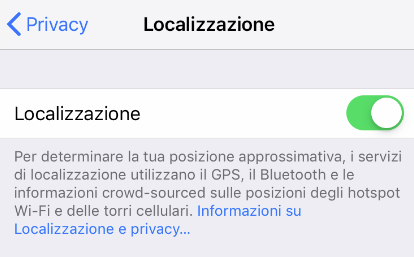
\includegraphics[]{abilita_gps.png}
\end{figure} 

\item Sempre nella stessa sezione si danno i permessi all'applicazione Safari di utilizzare tale servizio;

\begin{figure}[H]
	\centering
	\caption{Impostazione che permette tramite spunta di selezionare la voce Mentre si usa l'app}
	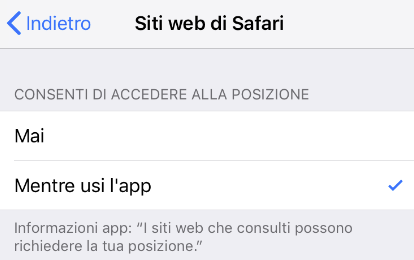
\includegraphics[]{safari_gps1.png}
\end{figure} 

\begin{figure}[H]
	\centering
	\caption{Dimostrazione della corretta procedura, Safari ha ora ottenuto i permessi}
	
\includegraphics[]{safari_gps2.png}
\end{figure} 


\item Sempre dalle impostazioni del dispositivo, selezionando safari è possibile abilitare l'utilizzo della fotocamera spuntando la relativa voce. (Questo passaggio è essenziale affinché nel front-end basic funzioni la parte per scattare una foto);
\begin{figure}[h]
	\centering
	\caption{Impostazioni che permettono tramite spunta delle voci 'Microfono e Fotocamera', di abilitare tali servizi}
	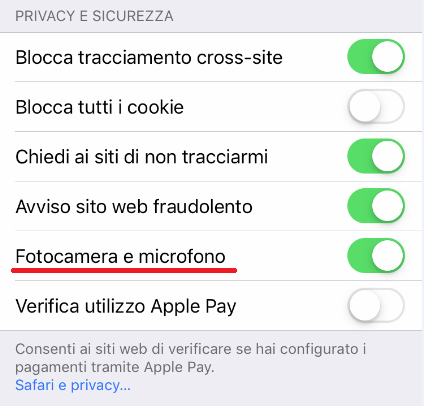
\includegraphics[scale=0.8]{fotocamera_safari.png}
\end{figure} 
\item Aprire l'ultima voce della sezione di Safari (Avanzate) e abilitare la voce \textbf{JavaScript};
\begin{figure}[h]
	\centering
	\caption{Impostazione che permette tramite spunta di abilitare le funzionalità 'JavaScript'}
	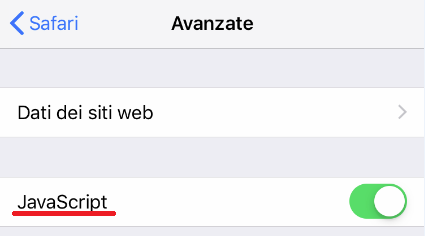
\includegraphics[scale=0.8]{safari_javascript.png}
\end{figure} 

\item A questo punto il dispositivo è settato correttamente e per accedere al sito si deve utilizzare il protocollo \textbf{HTTPS} e non il protocollo HTTP (altrimenti le API non funzionerebbero).

\end{itemize}

\section{Navigazione dell'applicazione Web}

\subsection{Full Front-End}
\subsubsection{Richiesta di Localizzazione}
\begin{figure}[H]
	\centering
	\caption{Richiesta di Localizzazione da parte dell'API, accettando si acconsente a condividere la proprio posizione affinché l'applicazione web funzioni correttamente.}
	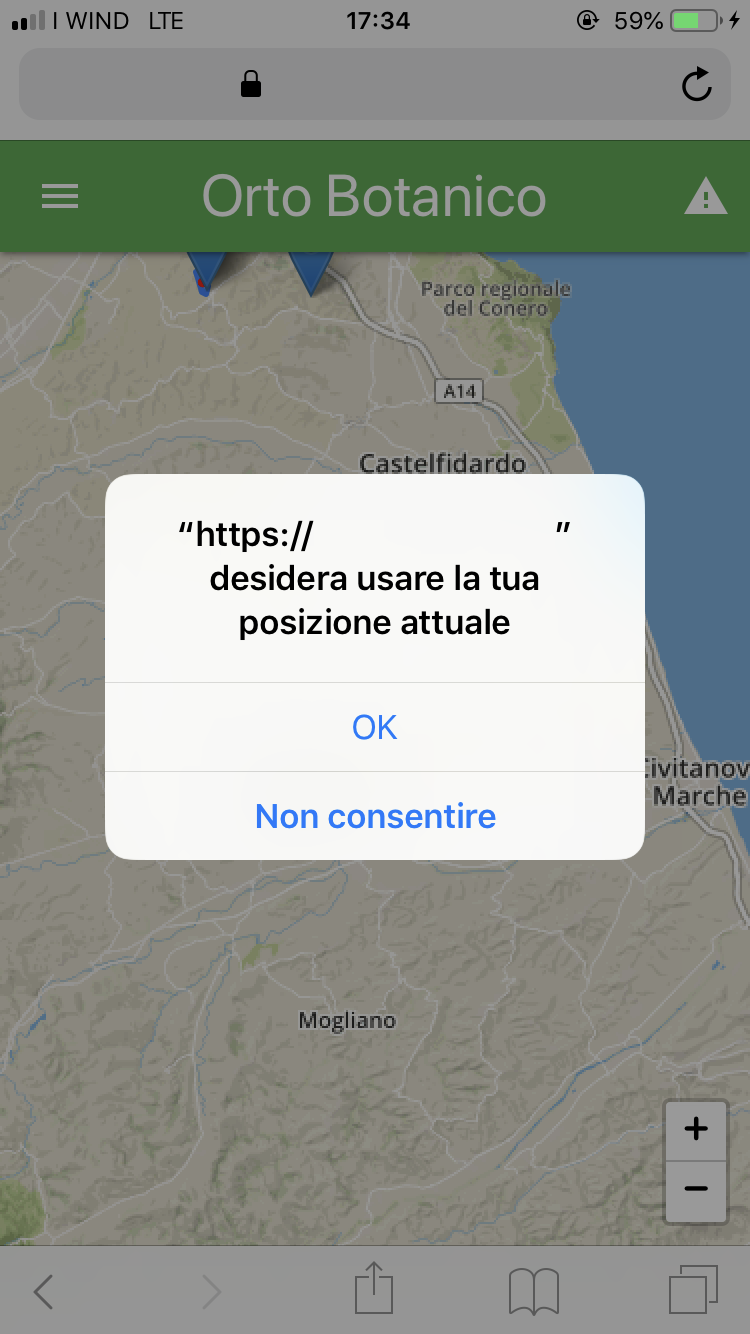
\includegraphics[scale=0.3]{location_request.png}
\end{figure} 
\newpage
\subsubsection{Homepage}
\begin{figure}[H]
	\centering
	\caption{Come si presenta l'homepage dell'applicazione Web con il front end full} 
	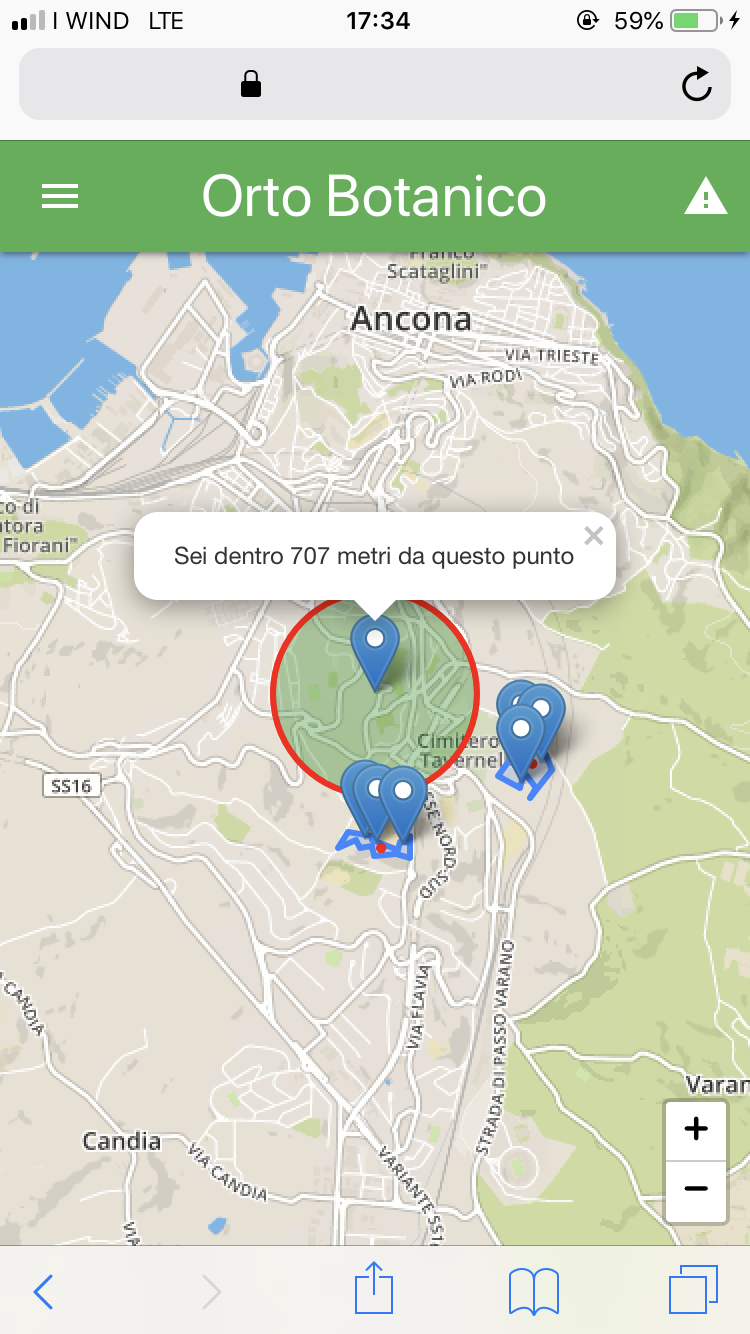
\includegraphics[scale=0.3]{homepage.png}
\end{figure} 
\newpage

\subsubsection{Sidebar}
\begin{figure}[H]
	\centering
	\caption{Come si presenta la sidebar di questo front end}
	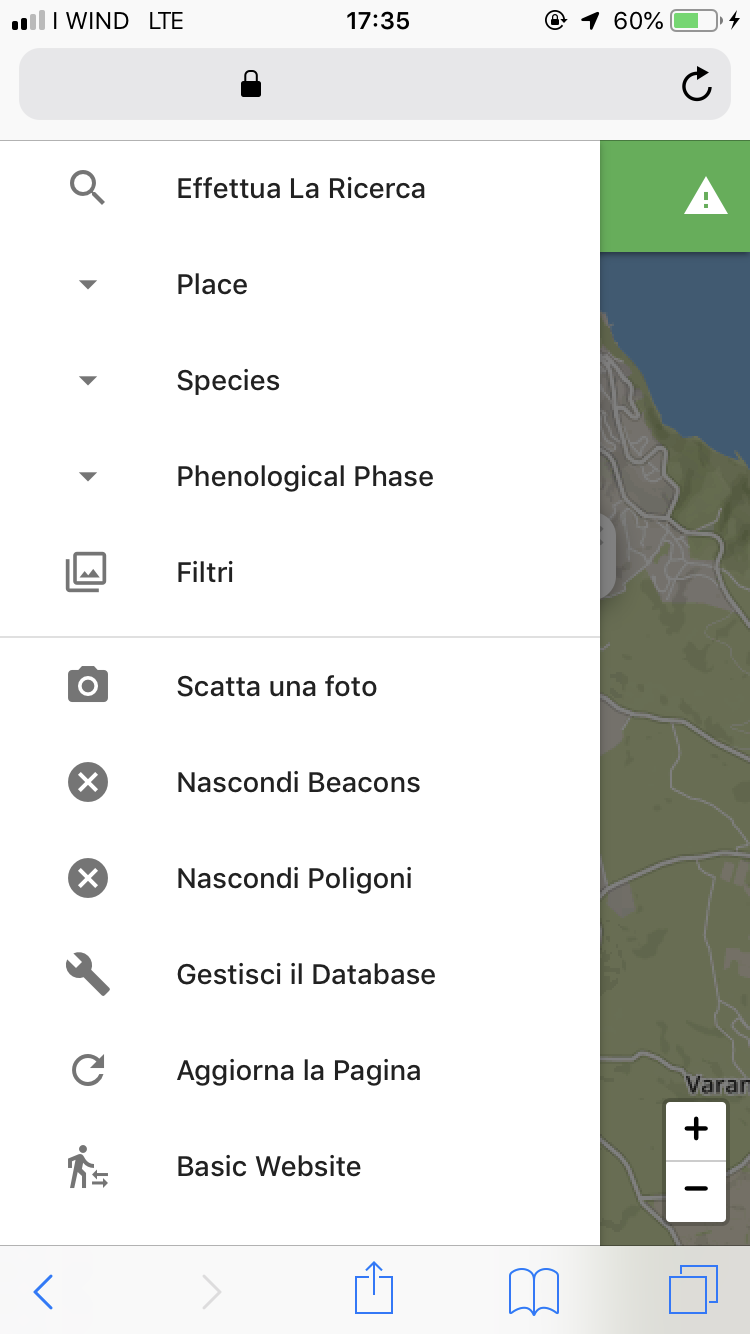
\includegraphics[scale=0.3]{sidebar.png}
\end{figure} 
\newpage

\subsubsection{Form Modale al click del Beacon}
\begin{figure}[H]
	\centering
	\caption{Ecco come si presenta la form che viene mostrata al click del beacon sulla mappa}
	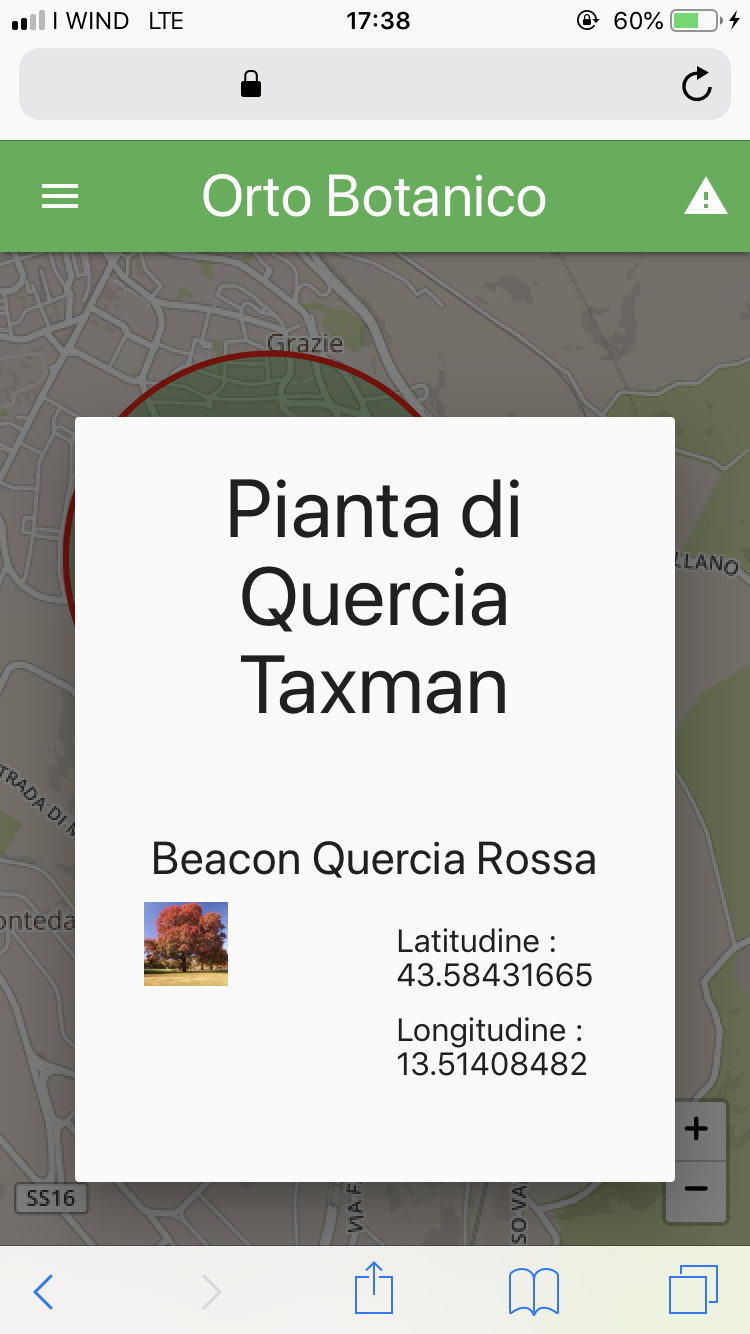
\includegraphics[scale=0.3]{beacon_popup.png}
\end{figure} 
\newpage

\subsubsection{Material Box della Form Modale del Beacon}
\begin{figure}[h]
	\centering
	\caption{Ecco come si presenta la Material Box (Light Box) al click dell'immagine della finestra modale del beacon}
	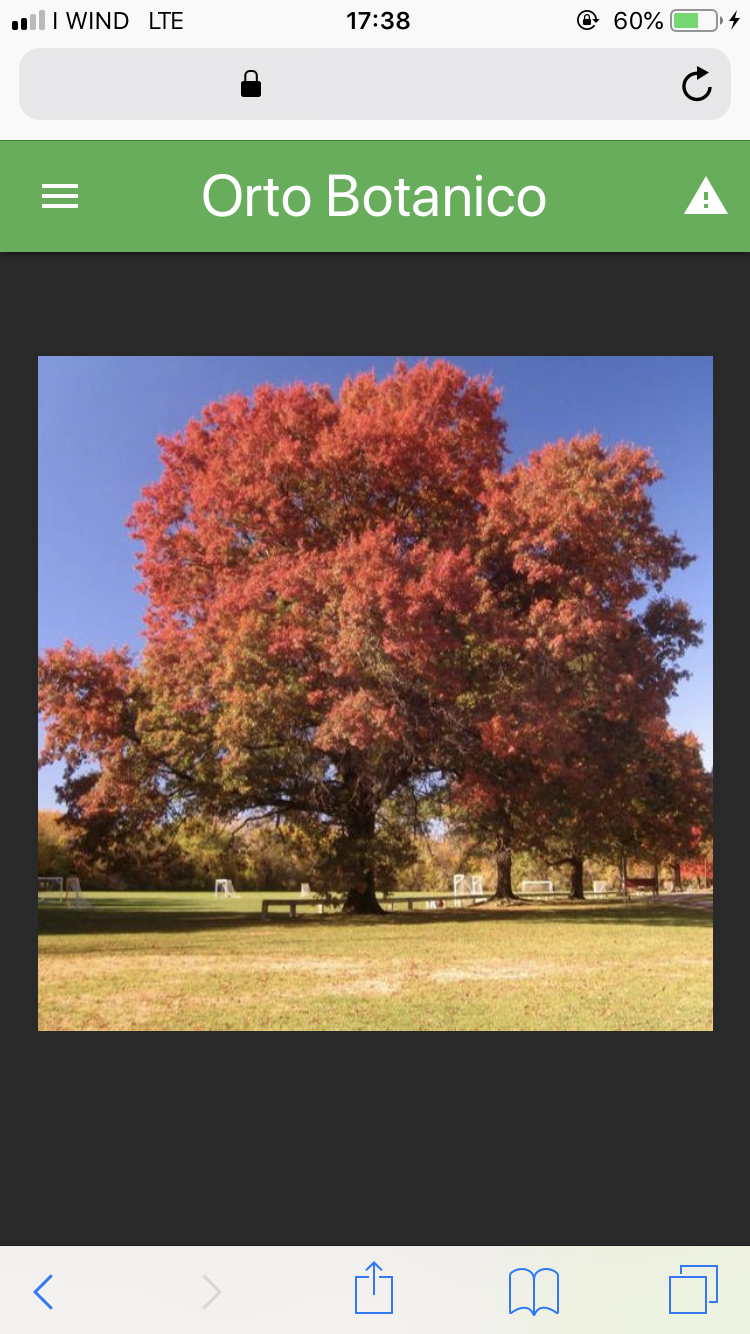
\includegraphics[scale=0.3]{material_box.png}
\end{figure} 
\newpage


\subsection{Basic Front-End}

\subsubsection{Homepage}
\begin{figure}[h]
	\centering
	\caption{Come si presenta l'homepage dell'applicazione Web con il front end basic}
	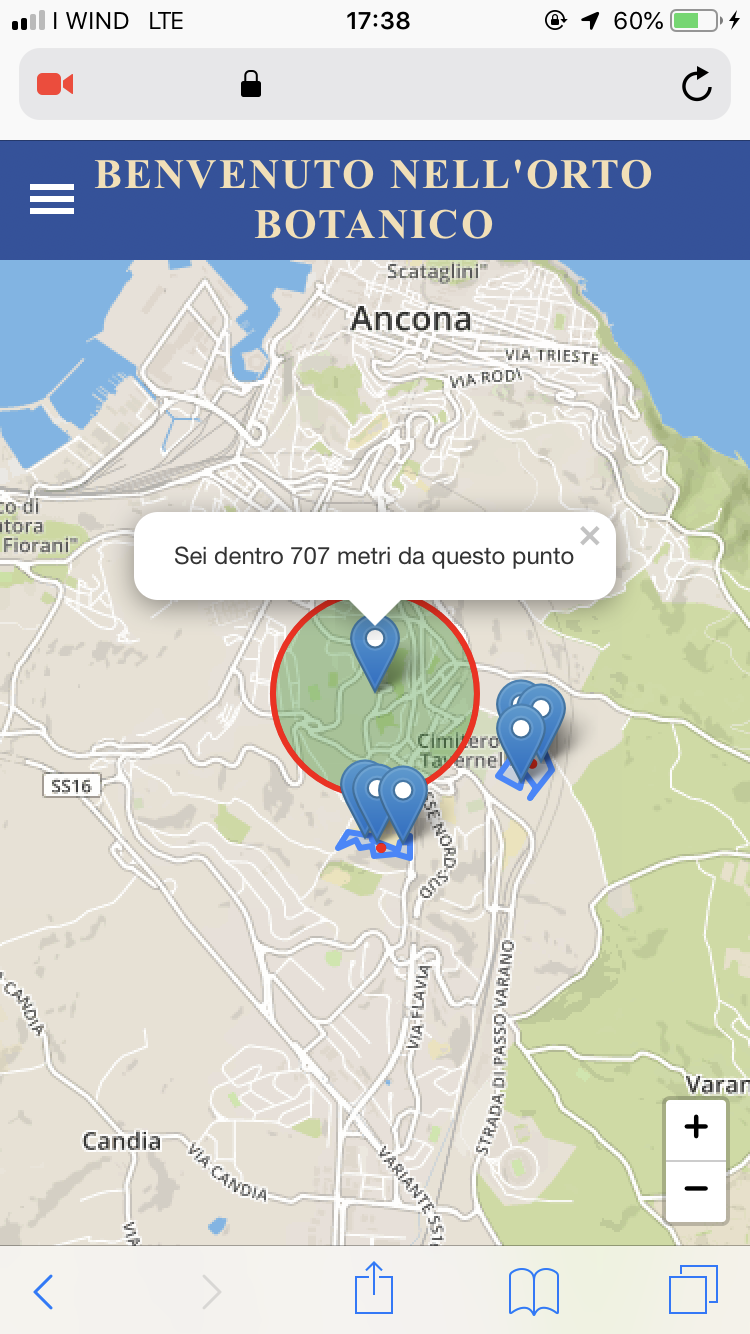
\includegraphics[scale=0.3]{homepage_basic.png}
\end{figure} 
\newpage

\subsubsection{Sidebar}
\begin{figure}[h]
	\centering
	\caption{Come si presenta la sidebar di questo front end}
	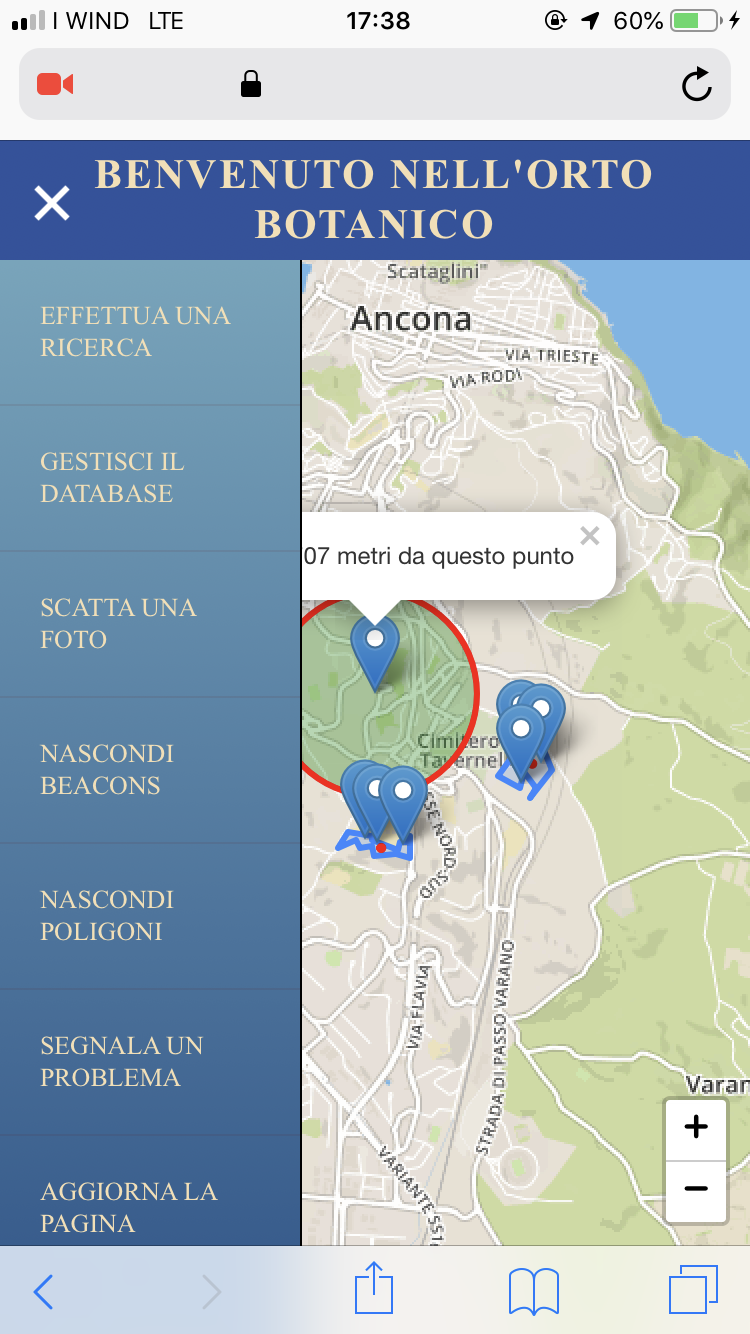
\includegraphics[scale=0.3]{sidebar_basic.png}
\end{figure} 
\newpage

\subsubsection{Finestra Modale per scattare Foto}
\begin{figure}[h]
	\centering
	\caption{Come si presenta la form modale per scattare le foto.}
	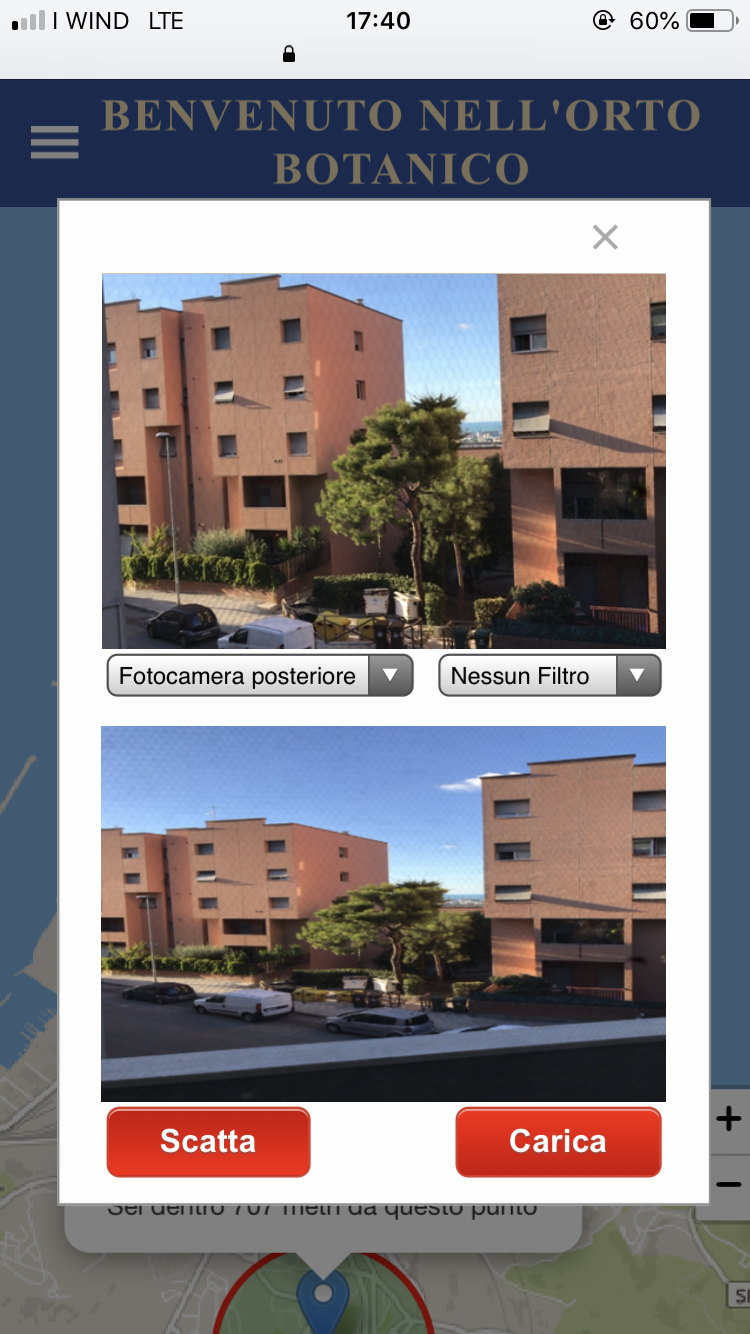
\includegraphics[scale=0.3]{canvas.png}
\end{figure} 
\newpage

 \clearemptydoublepage
\chapter{Conclusioni e Sviluppi Futuri}

\section{Conclusioni}
Lo sviluppo dell'applicazione web, secondo gli obiettivi fissati, è stato eseguito con successo. Per realizzare questo progetto sono stati utilizzati vari linguaggi e tecniche di programmazione che utilizzati insieme hanno portato a questo risultato. Tuttavia si sarebbero potuti utilizzare differenti approcci e differenti ambienti di sviluppo integrato per realizzare questo applicativo. Tali ambienti sarebbero potuti essere Xamarin, Mono, Android Studio o altri ancora.
\newline
L'applicazione web presenta, per come è stata fatta, un grande margine di miglioramento. Possono essere fatte molte implementazioni di nuove funzioni; ora andremo a vedere quali potrebbero essere.
\section{Sviluppi futuri}
\subsection{Implementazione AJAX}
Utilizzando l'applicazione web, notiamo subito che essa non è interattiva, cioè non aggiorna automaticamente i dati se non eseguendo un refresh. Un miglioramento consistente sarebbe implementare una logica di aggiornamento instantaneo della mappa utilizzando l'AJAX. In questo modo qulunque modifica fatta dal pannello di amministrazione (\textit{manage.php}) viene mostrata istantaneamente sulla mappa senza eseguire un refresh della pagina. \newline Ciò serve per avere una corretta visualizzazione in tempo reale dei dati, in modo da tener sempre aggiornati gli utenti per eventuali modifiche e aggiornamenti.
\subsection{Implementazione logica admin-staff-user}
Un altro accorgimento che si fa utilizzando l'applicazione web è l'impossibilità di avere un proprio account. 
Questo tipo di struttura per l'autenticazione mira ad implementare un sistema di accesso basato su 3 livelli: \textbf{user},\textbf{staff} e \textbf{admin}.
Si dovrà poi inserire un pannello per la registrazione di account user e un pannello di registrazione per account staff nella pagina \textit{manage.php}. Inoltre si implementa un sistema di notifiche. \newline
Dopo l'autenticazione ogni tipo di account avrà a disposizione un'area riservata come segue:
\begin{itemize}
\item \textbf{user} : la possibilità di salvare orti o piante di interesse, in modo da ottenere notifiche per le fioriture;
\item \textbf{staff} : questo tipo di account può accedere ad alcune funzioni del pannello di controllo (\textit{manage.php}) quali l'inserimento di beacon sulla mappa, il caricamento di immagini, lettura dei report e l'utilizzo di una nuova funzione (non implementata al momento) che permetta di associare un beacon ad un pianta;
\item \textbf{admin} : controllo generale del pannello \textit{manage.php} e l'implementazione di una nuova sezione volta a creare utenti nel database;
\end{itemize}
\subsection{Più funzioni in manage.php per manipolare i dati nel database}
Un altro aspetto futuro l'implementazione di una sezione nella pagina \textit{manage.php} in grado di effettuare ulteriori manipolazioni al database, quali:
\begin{itemize}
\item possibilità di eseguire codice SQL tramite un editor creato ad hoc. (Per esempio per la creazione delle tabelle);
\item possibilità di specificare i parametri di connessione e non renderli statici dal file \textit{config.php} (in modo da connettersi anche ad altri database);
\item possibilità di esportare un backup del database;
\item possibilità di importare un backup del database per effettuare un ripristino dei dati;
\item possibilità di creare in maniera guidata delle viste;
\item possibilità di creare in maniera guidata delle function;
\item possibilità di creare in maniera guidata delle stored procedures;
\item possibilità di creare in maniera guidata degli indici.
\end{itemize}
\section{Correzione dei BUG riscontrati}
Durante lo sviluppo, si sono riscontrati svariati bug con l'utilizzo dell'API per gestire la fotocamera dei dispositivi, verranno elencati i più rilevanti:
\begin{itemize}
\item non funziona con il browser Google Chrome da mobile (versione rilasciata in data 06/2018);
\item per cambiare fotocamera da quella anteriore a quella posteriore si deve utilizzare il menù a tendina svariate volte prima che abbia effetto;
\item la funzione \textit{drawImage}, che riceve in input l'immagine in streaming al momento dello pressione del bottone \textit{Scatta} dall'API, permette di disegnare l'immagine sul canvas, presenta un grave problema di resizing come è possibile vedere dalla figura \textbf{5.1.3}.
\end{itemize}
\section{Ottimizzazione del Codice}
Per quanto riguarda il codice, si potrebbero usare diversi approcci per avere più pulizia e efficienza. Dato che non era questo il concept del progetto, verranno ora elencati alcuni accorgimenti possibili per ottimizzare l'efficienza dell'applicazione web.
Si può approccio per la gestione degli eventi come definito nella sezione 3.3.6.1 separando le funzionalità delle struttura/contenuto e presentazione della pagine web. \newline
Dunque eliminando tutti gli \textit{onclick} e utilizzare \textit{addEventListener} nella pagina \textit{manage.php}.
\section{Altri accorgimenti futuri}
Un possibile accorgimento futuro per rendere l'applicazione web più professionale e desiderabile online è quella di acquistare un dominio, in modo che per raggiungere l'applicazione web si utilizza un'etichetta al posto dell'indirizzo ip. \newline
Un altro accorgimento è quello di acquistare un certificato in modo che ci si possa connettere all'applicazione web da browser utilizzando una connessione sicura (Https).

 \clearemptydoublepage

\nocite{*}
\bibliographystyle{plain}
\bibliography{Tesi}


\clearemptydoublepage

\listoffigures

\clearemptydoublepage





\end{document}
